% Options for packages loaded elsewhere
% Options for packages loaded elsewhere
\PassOptionsToPackage{unicode}{hyperref}
\PassOptionsToPackage{hyphens}{url}
\PassOptionsToPackage{dvipsnames,svgnames,x11names}{xcolor}
%
\documentclass[
  letterpaper,
  12pt]{article}
\usepackage{xcolor}
\usepackage[margin=1in]{geometry}
\usepackage{amsmath,amssymb}
\setcounter{secnumdepth}{-\maxdimen} % remove section numbering
\usepackage{iftex}
\ifPDFTeX
  \usepackage[T1]{fontenc}
  \usepackage[utf8]{inputenc}
  \usepackage{textcomp} % provide euro and other symbols
\else % if luatex or xetex
  \usepackage{unicode-math} % this also loads fontspec
  \defaultfontfeatures{Scale=MatchLowercase}
  \defaultfontfeatures[\rmfamily]{Ligatures=TeX,Scale=1}
\fi
\usepackage{lmodern}
\ifPDFTeX\else
  % xetex/luatex font selection
  \ifLuaTeX
    \usepackage{luaotfload}
    \directlua{luaotfload.add_fallback("mainfontfallback",{
      "LatinModernMath-Regular:mode=base;","DejaVuSans:mode=node;"
    })}
  \fi
  \setmainfont[,RawFeature={fallback=mainfontfallback}]{TeX Gyre Termes}
\fi
% Use upquote if available, for straight quotes in verbatim environments
\IfFileExists{upquote.sty}{\usepackage{upquote}}{}
\IfFileExists{microtype.sty}{% use microtype if available
  \usepackage[]{microtype}
  \UseMicrotypeSet[protrusion]{basicmath} % disable protrusion for tt fonts
}{}
% Make \paragraph and \subparagraph free-standing
\makeatletter
\ifx\paragraph\undefined\else
  \let\oldparagraph\paragraph
  \renewcommand{\paragraph}{
    \@ifstar
      \xxxParagraphStar
      \xxxParagraphNoStar
  }
  \newcommand{\xxxParagraphStar}[1]{\oldparagraph*{#1}\mbox{}}
  \newcommand{\xxxParagraphNoStar}[1]{\oldparagraph{#1}\mbox{}}
\fi
\ifx\subparagraph\undefined\else
  \let\oldsubparagraph\subparagraph
  \renewcommand{\subparagraph}{
    \@ifstar
      \xxxSubParagraphStar
      \xxxSubParagraphNoStar
  }
  \newcommand{\xxxSubParagraphStar}[1]{\oldsubparagraph*{#1}\mbox{}}
  \newcommand{\xxxSubParagraphNoStar}[1]{\oldsubparagraph{#1}\mbox{}}
\fi
\makeatother


\usepackage{longtable,booktabs,array}
\newcounter{none} % for unnumbered tables
\usepackage{calc} % for calculating minipage widths
% Correct order of tables after \paragraph or \subparagraph
\usepackage{etoolbox}
\makeatletter
\patchcmd\longtable{\par}{\if@noskipsec\mbox{}\fi\par}{}{}
\makeatother
% Allow footnotes in longtable head/foot
\IfFileExists{footnotehyper.sty}{\usepackage{footnotehyper}}{\usepackage{footnote}}
\makesavenoteenv{longtable}
\usepackage{graphicx}
\makeatletter
\newsavebox\pandoc@box
\newcommand*\pandocbounded[1]{% scales image to fit in text height/width
  \sbox\pandoc@box{#1}%
  \Gscale@div\@tempa{\textheight}{\dimexpr\ht\pandoc@box+\dp\pandoc@box\relax}%
  \Gscale@div\@tempb{\linewidth}{\wd\pandoc@box}%
  \ifdim\@tempb\p@<\@tempa\p@\let\@tempa\@tempb\fi% select the smaller of both
  \ifdim\@tempa\p@<\p@\scalebox{\@tempa}{\usebox\pandoc@box}%
  \else\usebox{\pandoc@box}%
  \fi%
}
% Set default figure placement to htbp
\def\fps@figure{htbp}
\makeatother


% definitions for citeproc citations
\NewDocumentCommand\citeproctext{}{}
\NewDocumentCommand\citeproc{mm}{%
  \begingroup\def\citeproctext{#2}\cite{#1}\endgroup}
\makeatletter
 % allow citations to break across lines
 \let\@cite@ofmt\@firstofone
 % avoid brackets around text for \cite:
 \def\@biblabel#1{}
 \def\@cite#1#2{{#1\if@tempswa , #2\fi}}
\makeatother
\newlength{\cslhangindent}
\setlength{\cslhangindent}{1.5em}
\newlength{\csllabelwidth}
\setlength{\csllabelwidth}{3em}
\newenvironment{CSLReferences}[2] % #1 hanging-indent, #2 entry-spacing
 {\begin{list}{}{%
  \setlength{\itemindent}{0pt}
  \setlength{\leftmargin}{0pt}
  \setlength{\parsep}{0pt}
  % turn on hanging indent if param 1 is 1
  \ifodd #1
   \setlength{\leftmargin}{\cslhangindent}
   \setlength{\itemindent}{-1\cslhangindent}
  \fi
  % set entry spacing
  \setlength{\itemsep}{#2\baselineskip}}}
 {\end{list}}
\usepackage{calc}
\newcommand{\CSLBlock}[1]{\hfill\break\parbox[t]{\linewidth}{\strut\ignorespaces#1\strut}}
\newcommand{\CSLLeftMargin}[1]{\parbox[t]{\csllabelwidth}{\strut#1\strut}}
\newcommand{\CSLRightInline}[1]{\parbox[t]{\linewidth - \csllabelwidth}{\strut#1\strut}}
\newcommand{\CSLIndent}[1]{\hspace{\cslhangindent}#1}



\setlength{\emergencystretch}{3em} % prevent overfull lines

\providecommand{\tightlist}{%
  \setlength{\itemsep}{0pt}\setlength{\parskip}{0pt}}



 


% APA Seventh Edition styling, in plain LaTeX.
%
% Everything here is ordinary article-class styling. There is no apa7: the
% title page, the abstract, the author note and the notes below floats all
% arrive as ordinary blocks from apaquarto's filters, and this file only says
% how they are set. Each command below is used by formatlatex.lua.

% The colour typst gives a link, which is its own named blue. The .pdf
% asks for it by name in _extension.yml; the name has to exist before
% pandoc's own hypersetup names it, and this file is read first.
\definecolor{apalink}{HTML}{0074D9}
% A link inside one of the lists takes the colour of the text around it,
% which is what typst's outlines do with theirs. toccolor overrides it:
% pandoc's latex template writes no toccolor of its own, so the lists
% being apaquarto's own means honouring it here. formatlatex.lua
% renews this when a document names one.
\definecolor{apatext}{HTML}{000000}
\newcommand{\apatoccolor}{apatext}

% How many levels of heading the contents lists, which is quarto's
% toc-depth. The article class counts three of its own accord;
% formatlatex.lua renews this where a document asks for another number.
\newcommand{\apatocdepth}{3}

\usepackage{setspace}
\usepackage{fancyhdr}
\usepackage{titlesec}
\usepackage{ragged2e}
\usepackage{etoolbox}
% The orcid mark in the author note, drawn in tex and linked to the orcid.
% frontmatter.lua writes \orcidlink{...} for this format instead of placing
% the svg apaquarto ships, which quarto would have to put through
% rsvg-convert -- absent on linux, where the render then stops.
% apa7 does the same thing with its own addORCIDlink.
\usepackage{orcidlink}

% [H] placement, which floatsintext asks for
\usepackage{float}

% --- Page and paragraph -----------------------------------------------------
% APA: double spaced throughout, first line of every paragraph indented half an
% inch, no extra space between paragraphs, text flush left with a ragged right
% edge rather than justified.
% \RaggedRight sets \parindent to \RaggedRightParindent, so the indent has to
% be told to it before it is switched on. Setting \parindent afterwards instead
% leaves every paragraph flush left.
%
% ragged2e's \RaggedRight lets a line fall short of the measure by at most
% 2em, so where the next word does not fit TeX breaks it at a hyphen instead.
% APA asks for no hyphenation at the ends of lines. An infinite stretch, which
% is what LaTeX's own \raggedright has, leaves a short line rather than a
% broken word. The length is read when \RaggedRight is switched on, so it is
% set before.
\setlength{\parindent}{0.5in}
\setlength{\parskip}{0pt}
\setlength{\RaggedRightParindent}{0.5in}
\setlength{\RaggedRightRightskip}{0pt plus 1fil}
\RaggedRight

% setspace's own double spacing, which is what apa7 uses and which comes to
% about twice the font size. Asking for linestretch: 2 instead multiplies the
% normal baseline skip, which is already larger than the font size, and set the
% lines about a fifth further apart than apaquarto-pdf sets them.
\doublespacing

% --- Running head -----------------------------------------------------------
% APA seventh edition: the short title in capitals at the left of every page
% and the page number at the right. No rule under it.
\pagestyle{fancy}
\fancyhf{}
\renewcommand{\headrulewidth}{0pt}
\fancyhead[L]{\apashorttitle}
\fancyhead[R]{\thepage}
\newcommand{\apashorttitle}{}
\newcommand{\setapashorttitle}[1]{\renewcommand{\apashorttitle}{\MakeUppercase{#1}}}
\newcommand{\apaauthorline}{}
\newcommand{\setapaauthorline}[1]{\renewcommand{\apaauthorline}{\MakeUppercase{#1}}}

% The head a published article carries, which is the one apaquarto's typst
% format sets: the short title centred on a recto page and the authors'
% surnames centred on a verso one, both in capitals, with the page number in
% the outer corner. The head is smaller than the body and the page number is
% not, which is how the journals set it.
%
% Recto and verso only differ once the document is twoside, which
% formatlatex.lua asks for along with this.
\newcommand{\apaheadsize}{\fontsize{8}{10}\selectfont}
\newcommand{\apajournalhead}{%
  \fancyhf{}%
  \fancyhead[LE]{\thepage}%
  \fancyhead[RO]{\thepage}%
  \fancyhead[CE]{{\apaheadsize\apaauthorline}}%
  \fancyhead[CO]{{\apaheadsize\apashorttitle}}}

% The head a student paper carries: the page number and nothing else. APA
% seventh edition drops the running head from student work, which is what
% apaquarto's typst format does and what the apa7 class did for the .pdf
% before 6.0.0 stopped using it. Issue #166.
\newcommand{\apastudenthead}{%
  \fancyhf{}%
  \fancyhead[R]{\thepage}}

% The head a dissertation carries, which is none. The Temple University
% Graduate School's handbook asks for the page number and nothing else, and
% the dissertations it publishes set it at the centre of the foot. The title
% page is counted but not numbered, which \thispagestyle{empty} does where the
% page is built.
\newcommand{\apathesishead}{%
  \fancyhf{}%
  \fancyfoot[C]{\thepage}}

% The leader dots of a table of contents, set closer together than \dotfill
% sets them. \dotfill leaves 0.44em between dots, which reads as a dotted
% line rather than as a leader; a contents wants them tighter, and tighter is
% what the Graduate School's own template shows.
\makeatletter
\newcommand{\apadotfill}{%
  \leavevmode\cleaders\hb@xt@ .3em{\hss.\hss}\hfill\kern\z@}
\makeatother

% Float placement in a published article.
%
% A float spanning both columns can only go at the top of a page, at the foot
% of one where stfloats allows it, or on a page of its own. Latex's own
% fractions are cautious enough that the two spanning floats in example.qmd
% went to a page of their own with no text on it at all, where apa7 and the
% typst format both set them at the head of a page of text. A spanning float
% may now take nine tenths of the top of a page, and a float page has to be
% nine tenths full before latex will make one.
\newcommand{\apajoufloats}{%
  \renewcommand{\dbltopfraction}{0.9}%
  \renewcommand{\dblfloatpagefraction}{0.9}%
  \renewcommand{\topfraction}{0.9}%
  \renewcommand{\bottomfraction}{0.5}%
  \renewcommand{\textfraction}{0.07}%
  \renewcommand{\floatpagefraction}{0.85}%
  \setcounter{dbltopnumber}{2}%
  \setcounter{topnumber}{3}%
  \setcounter{totalnumber}{5}}

% The gutter between the columns, which typst leaves at a twenty-fifth of the
% text width and latex at ten points.
\newcommand{\apajoucolumnsep}{\setlength{\columnsep}{0.04\textwidth}}

% The first page of a journal or document paper carries the masthead instead of
% a running head, so it is left plain.
\fancypagestyle{apafirstpage}{%
  \fancyhf{}%
  \renewcommand{\headrulewidth}{0pt}}

% The opening page of a published article also carries its number at the centre
% of the bottom margin, where the running head has not started yet. Every
% journal APA prints does this; the Journal of Educational Psychology, which
% this mode is measured against, sets it at the running head's own size rather
% than the larger size it gives the number in the head.
%
% The opening page only. From the second page on the number is in the head, in
% the outer corner, and a second one at the foot would be one too many.
\fancypagestyle{apajoufirstpage}{%
  \fancyhf{}%
  \renewcommand{\headrulewidth}{0pt}%
  \fancyfoot[C]{{\apaheadsize\thepage}}}

% Two columns, which is what a published article is set in. \twocolumn starts a
% page, so it is asked for at the start of the document rather than in the
% preamble, where it would be too early to take effect.
\newcommand{\apatwocolumn}{\AtBeginDocument{\twocolumn}}

% --- Journal front matter ---------------------------------------------------
% In a published article the title, the byline, the abstract and the lines
% under them span the page beneath the masthead rather than standing in the
% first column, and the author note goes to the foot of that column. The sizes
% are the ones apa7 gives its journal mode, which is where apaquarto's typst
% format takes them from as well: at a 10pt base the title is \LARGE and
% unemphasised, the byline \large, the affiliations the body size, and the
% abstract and everything with it \small.
\newcommand{\apajoutitle}[1]{%
  {\centering\fontsize{17.28}{20.74}\selectfont #1\par}}

% The byline, with the affiliations under it at the body size. formatlatex.lua
% switches to the smaller size after the first paragraph, which is the byline.
% The gaps between the parts of the front matter are measured against the
% typst masthead, which is what this page is meant to look like.
\newenvironment{apajoubyline}
  {\par\vspace{9pt}\centering\fontsize{12}{14}\selectfont}
  {\par}
\newcommand{\apajouaffiliationsize}{\fontsize{10}{12}\selectfont}

% The abstract, the impact statement and the lines under them: smaller, and in
% a block narrower than the masthead, centred under the byline. apa7 sets its
% journal abstract in a 4.6875in parbox, which is where the width comes from.
% The text inside is justified, like the body of the article below it.
\newlength{\apajounarrowwidth}
\setlength{\apajounarrowwidth}{4.6875in}
% parskip as well as leading: typst leaves a line and a bit between the
% keywords and the supplemental materials under them, where latex on its own
% would leave only the line.
\newenvironment{apajounarrow}
  {\par\vspace{7pt}\centering
   \begin{minipage}{\apajounarrowwidth}%
   \fontsize{9}{11}\selectfont
   \setlength{\parskip}{6pt}%
   \setlength{\JustifyingParindent}{0pt}\justifying\setlength{\parindent}{0pt}}
  {\end{minipage}\par\vspace{10pt}}

% The impact statement, ruled off from the abstract above it and the keywords
% below it. The same box the typst masthead draws: a half-point rule 6pt clear
% of the text on every side, with 9pt above and below.
\newsavebox{\apajouimpactbox}
\newenvironment{apajouimpact}
  {\par\vspace{3pt}%
   \setlength{\fboxrule}{0.5pt}\setlength{\fboxsep}{6pt}%
   \begin{lrbox}{\apajouimpactbox}%
   \begin{minipage}{\dimexpr\linewidth-2\fboxsep-2\fboxrule\relax}}
  {\end{minipage}\end{lrbox}%
   \noindent\fbox{\usebox{\apajouimpactbox}}\par\vspace{3pt}}

% The orcid lines of the author note. Each is one short name-and-link
% paragraph, so justifying it stretches the gaps across the measure and
% indenting it leaves the names out of line with each other. They are set
% flush left and unindented, while the prose paragraphs of the note keep the
% indent they are given, which is what the typst masthead does with them.
\newenvironment{apajouorcid}
  {\par\setlength{\parindent}{0pt}%
   \setlength{\RaggedRightParindent}{0pt}\RaggedRight}
  {\par}

% The author note, at the foot of the first page under a rule.
%
% A journal sets a short note at the foot of the first column and a long one
% across the foot of the page. apaquarto's typst format measures the note and
% does both, and so does this: the note is set once into a box the width of a
% column, and if it fits in a third of the text height it stays in that box at
% the foot of the column. A longer one is set again across the page, since a
% note that fills a column leaves the article nowhere to start.
%
% A third of the text height is the share typst measures against, and it is
% also about what latex will hold at the foot of a column: bottomfraction is
% half a page in journal mode, so a note under a third always fits and never
% drifts to a later page.
%
% The environment collects its body so that it can be set twice, which is what
% environ is for. A footnote would be the natural way to put something at the
% foot of a column, but latex sets a footnote only if it fits the column it was
% raised in and breaks it across pages otherwise, and on a page of floats that
% sent the output routine round in circles.
%
% stfloats is what allows a float spanning both columns to be set at the foot
% of a page. Latex on its own will only put one at the top, and silently drops
% a starred float asked for anywhere else.
\usepackage{stfloats}
\usepackage{environ}
\newlength{\apajounoteindent}
\setlength{\apajounoteindent}{1.1em}
\newsavebox{\apajounotebox}

% Justified, like the body of the article above it. The orcid lines inside
% the note are not: apajouorcid sets them flush left again, since justifying
% one short name-and-link paragraph stretches its gaps across the measure.
\newcommand{\apajounotetext}{%
  \fontsize{9}{11}\selectfont
  \setlength{\JustifyingParindent}{\apajounoteindent}%
  \justifying
  \setlength{\parindent}{\apajounoteindent}}

\newcommand{\apajounoterule}{%
  \noindent\rule{\linewidth}{0.5pt}%
  \par\vspace{\dimexpr0.4em+3pt\relax}}

\NewEnviron{apajounote}{%
  \sbox{\apajounotebox}{%
    \begin{minipage}{\columnwidth}%
      \apajounotetext\BODY
    \end{minipage}}%
  \ifdim\dimexpr\ht\apajounotebox+\dp\apajounotebox\relax>\dimexpr\textheight/3\relax
    \begin{figure*}[b]%
      \apajounoterule
      \apajounotetext\BODY
    \end{figure*}%
  \else
    \begin{figure}[b]%
      \apajounoterule
      \usebox{\apajounotebox}%
    \end{figure}%
  \fi}

% --- Lists of figures and tables ---------------------------------------------
% APA sets these as a plain list: the float's name and its title on one line,
% then a leader out to the page number. Nothing is indented and nothing is
% numbered again -- floatlatex.lua has already written each line as "Figure 1.
% The Figure Caption", the line the .docx and typst lists give, so latex has
% only to place it.
%
% \l@figure and \l@table are what \listoffigures and \listoftables use
% for each line, and \@dottedtocline is the class's own: it sets the text,
% fills out to the page number with dots, and hangs the turn-over lines. Its
% two lengths are the indent before the text and the room kept for a number
% in front of it. Both are zero, since the number is part of the text here
% and the class would otherwise indent the line and leave a gap for it.
\makeatletter
\renewcommand*\l@figure{\@dottedtocline{1}{0em}{0em}}
\let \l@table \l@figure
\makeatother

% The table of contents. Its lines are set like the lists of figures and
% tables above -- the heading, a leader, the page -- but indented a level at
% a time, which is what tells a subsection from a section.
\makeatletter
\renewcommand*\l@section{\@dottedtocline{1}{0em}{0em}}
\renewcommand*\l@subsection{\@dottedtocline{2}{1.5em}{0em}}
\renewcommand*\l@subsubsection{\@dottedtocline{3}{3em}{0em}}
\makeatother

% The headings of the three lists, which formatlatex.lua sets from the
% document's language.
\newcommand{\apacontentsname}{Table of Contents}
\newcommand{\apalistfigurename}{List of Figures}
\newcommand{\apalisttablename}{List of Tables}

\newcommand{\apatableofcontents}{%
  \begingroup
  \hypersetup{linkcolor=\apatoccolor,citecolor=\apatoccolor,urlcolor=\apatoccolor}%
  \renewcommand{\contentsname}{\apacontentsname}%
  \setcounter{tocdepth}{\apatocdepth}%
  \tableofcontents
  \endgroup}

% Whether a list starts a page of its own is formatlatex.lua's to say: it
% does in every mode but jou, where a published article runs the lists on
% in the columns as typst's journal mode does.
% The heading each list carries, set like any other section heading. The
% article class writes the heading itself from \listfigurename, so the name
% is set first and the list follows.
\newcommand{\apalistoffigures}{%
  \begingroup
  \hypersetup{linkcolor=\apatoccolor,citecolor=\apatoccolor,urlcolor=\apatoccolor}%
  \renewcommand{\listfigurename}{\apalistfigurename}%
  \listoffigures
  \endgroup}
\newcommand{\apalistoftables}{%
  \begingroup
  \hypersetup{linkcolor=\apatoccolor,citecolor=\apatoccolor,urlcolor=\apatoccolor}%
  \renewcommand{\listtablename}{\apalisttablename}%
  \listoftables
  \endgroup}

% --- Journal masthead -------------------------------------------------------
% The band a published article carries at the head of its first page: the
% journal's logo at the left with its name opposite, a rule under both, and the
% copyright on the left beneath it with the issue and the doi on the right.
% apaquarto's typst format sets the same band, measured off the Journal of
% Educational Psychology, and the sizes here are the ones named there: a 12pt
% name over 8pt metadata, a half-point rule, and a half-inch band the logo is
% fitted to whatever its proportions. The space around the rule and the
% leading of the metadata are not the values typst names -- see the two
% commands below, which say why.
%
% frontmatter.lua builds the masthead out of the four commands below and
% formatlatex.lua hands it to \twocolumn, which is the only thing that sets
% material across both columns of a two-column page.
\newlength{\apamastheadrulewidth}
\setlength{\apamastheadrulewidth}{0.5pt}
\newlength{\apalogoheight}
\setlength{\apalogoheight}{0.5in}
\newsavebox{\apamastheadbox}

% A journal sets its masthead above where the text of the page begins, so it is
% lifted into the top margin by half of that margin, which is what the typst
% format does. Written as half the distance from the top of the paper to the
% top of the text block, so that a document setting its own margin is followed
% rather than overruled.
%
% Half the margin above the running head would be the closer reading of what
% typst lifts by, and it puts the band within a point of typst's. It also
% makes the box that much taller, which pushes the title, the abstract and the
% first line of the body down by the same amount and puts all four of those
% out by eight points. The band is the part that can afford to be out: this
% sets it about five points higher than typst sets it, and everything under it
% level to the point.
\newcommand{\apamastheadlift}{%
  \vspace*{-\dimexpr(1in+\voffset+\topmargin+\headheight+\headsep)/2\relax}}

% Declarations rather than commands taking an argument: the metadata below is
% two lines with a break between them, which reads more plainly set into a
% paragraph than passed through a pair of braces.
\newcommand{\apamastheadname}{\fontsize{12}{14}\selectfont}
% 8pt on 10.75, which is the leading the typst masthead sets its two lines of
% metadata at. The 9.6 an 8pt size would take by the usual ratio set them a
% point and a quarter closer together than that.
\newcommand{\apamastheadsmall}{\fontsize{8}{10.75}\selectfont}

\newcommand{\apamastheadlogo}[1]{\includegraphics[height=\apalogoheight]{#1}}

% The logo and the journal's name, sitting on one baseline at either edge.
\newcommand{\apamastheadhead}[2]{%
  \noindent #1\hfill{\apamastheadname #2}\par}

% nointerlineskip on either side of the rule, and the space written out in
% full. A rule set as its own paragraph takes a whole line's leading above it
% and the metadata under it takes another, which put the rule a line lower
% than typst sets it and opened the band out by a line at each turn.
%
% The two lengths are not the 3pt the typst masthead names, because typst adds
% that to the space a grid row carries of its own and nointerlineskip here
% leaves none to add it to. They are measured instead: they put the rule and
% the first line of the metadata within a point of where the typst masthead
% puts them, which is what this band is meant to look like.
\newcommand{\apamastheadline}{%
  \par\nointerlineskip\vspace{5.5pt}%
  \noindent\rule{\linewidth}{\apamastheadrulewidth}%
  \par\nointerlineskip\vspace{6.5pt}}

% The copyright and the issn on the left, the issue and the doi on the right,
% each pair set as two lines. Half the measure each, less half the gutter the
% typst masthead leaves between them.
\newcommand{\apamastheadfoot}[2]{%
  \noindent
  \begin{minipage}[t]{\dimexpr0.5\linewidth-0.5em\relax}%
    \apamastheadsmall\raggedright #1%
  \end{minipage}\hfill
  \begin{minipage}[t]{\dimexpr0.5\linewidth-0.5em\relax}%
    \apamastheadsmall\raggedleft #2%
  \end{minipage}\par\vspace{1em}}

% The first-line indent of a published article, which is a good deal smaller
% than the half inch a manuscript takes: apa7 sets it at about 1.1 times the
% body size. Written in em so that it follows the type size, whatever the
% writer has asked for.
%
% The body of a published article is justified, where a manuscript is set
% flush left with a ragged right edge. The preamble asks for RaggedRight,
% which is right for the other three modes, so journal mode turns it back off
% with ragged2e's own \justifying.
%
% \justifying reads \JustifyingParindent the way \RaggedRight reads
% \RaggedRightParindent, so the length is set before it is switched on.
% \parindent is set as well, since the two are only kept in step by whichever
% of the pair was asked for last.
%
% Written into the body rather than the preamble. The half inch a manuscript
% takes is set further down the preamble than an in-header include reaches, so
% a preamble setting of this would simply be undone.
\newlength{\apajouparindent}
\setlength{\apajouparindent}{1.1em}
\newcommand{\apajournalindent}{%
  \setlength{\JustifyingParindent}{\apajouparindent}%
  \justifying
  \setlength{\parindent}{\apajouparindent}}

% booktabs' rules take an optional trim argument, written \midrule(rl), which
% they look for by peeking at the single character that follows the rule.
% Inside a longtable that peek is \@BLTrule's, and a table whose first cell
% opens with a literal ( -- the term name (Intercept), which every model
% summary produces -- is read as the start of a trim spec. booktabs then tries
% to parse the letters of Intercept as trim sides, leaves \cmrsideswitch
% undefined and takes the whole build down with "Undefined control sequence".
%
% Pandoc's own tables are out of reach of this, since it writes \noalign{}
% after every rule, but a table written as latex puts the row hard against the
% rule. Giving \@BLTrule an empty trim spec of its own stops it peeking; the
% trim argument is then unavailable inside longtables, which is no loss, since
% apaquarto never writes one.
%
% apa7 patches this in its header.tex partial, which this format has no part
% of, so it goes here. See tests/booktabs-paren-cell.qmd, and issue #164.
\makeatletter
\def\@BLTrule{\@@BLTrule()}
\makeatother

% A longtable refuses to be set in two columns, and quarto writes every
% markdown table as a longtable while flextable builds its tables out of one.
% A longtable earns its keep by breaking over pages, which a table inside a
% column cannot do anyway, so in two columns each one is set as an ordinary
% tabular instead: the row and rule syntax is the same.
%
% What the conversion has to get right is the four commands that mark a
% longtable's repeating head and foot. They do not merely say where the head
% and the foot end; they say which rows repeat on every page and which are set
% once, and in the source the foot stands above the body. Made to do nothing,
% as they were, every row was set where it stood: a table with a repeating
% head printed the head twice, a pandoc table printed its \bottomrule under
% the \midrule and had no rule at the foot, and a flextable printed its note
% row between the head and the body.
%
% So the head that repeats is thrown away, the first head being the one that
% is wanted, and the foot is collected and set at the end of the table where
% it belongs. Both grabs are \long, since the rows of a flextable have blank
% lines between them, and the one that saves the foot is wrapped in \noalign:
% an assignment between two rows would otherwise open a cell, and the row
% after it lost its first column.
\makeatletter
\newtoks\apa@lt@foot
\long\def\apa@lt@firsthead#1\endhead{\apa@lt@head}
\def\apa@lt@head{\apa@lt@grab}
\long\def\apa@lt@grab#1\endlastfoot{\noalign{\global\apa@lt@foot{#1}}}
\newcommand{\apalongtableastabular}{%
  \renewenvironment{longtable}[2][]{%
    \global\apa@lt@foot{}%
    \let\endfirsthead\apa@lt@firsthead
    \let\endhead\apa@lt@head
    \let\endfoot\relax
    \let\endlastfoot\relax
    \begin{tabular}{##2}%
  }{%
    \the\apa@lt@foot
    \end{tabular}%
    % The space after \end{longtable} ignored, as after a list or a
    % quotation. It sat on the tabular's line, and when the table ran the
    % full width of the page, as one with a column of text does, it went on
    % to a second, empty line, which set the note a point lower than under a
    % narrower table (tests/layout-table-rules.qmd).
    \global\@ignoretrue
  }}
\makeatother

% --- Headings ---------------------------------------------------------------
% titlespacing rather than titlespacing*: the starred form takes the indent off
% the paragraph that follows a heading, which is latex's habit and not APA's.
% APA indents the first line of every paragraph, the one under a heading along
% with the rest.
% The five APA levels. One to three are their own paragraphs; four and five run
% into the text that follows them, which is why they are set as runin.
% Numbering is off: APA headings are never numbered.
%
% No space is added above or below a heading: APA sets one on a line of its
% own in the line spacing of the text around it, as typst does. The space
% above was \baselineskip, which titlesec adds on top of the line spacing,
% so every heading stood a blank line below the text before it, 49pt from it
% in a manuscript where the lines are 24pt apart (tests/layout-manuscript.qmd).
\setcounter{secnumdepth}{-1}

\titleformat{\section}[block]
  {\normalfont\bfseries\centering}{}{0pt}{}
\titlespacing{\section}{0pt}{0pt}{0pt}

\titleformat{\subsection}[block]
  {\normalfont\bfseries\raggedright}{}{0pt}{}
\titlespacing{\subsection}{0pt}{0pt}{0pt}

\titleformat{\subsubsection}[block]
  {\normalfont\bfseries\itshape\raggedright}{}{0pt}{}
\titlespacing{\subsubsection}{0pt}{0pt}{0pt}

% No [.] suffix: apaheader.lua has already put a full stop at the end of a
% level four or five heading, and only when the heading did not end in one
% already. A stop added here as well doubled every one of them, and turned a
% heading ending in a question mark into "...?.".
\titleformat{\paragraph}[runin]
  {\normalfont\bfseries}{}{0pt}{}
\titlespacing{\paragraph}{\parindent}{0pt}{0.5em}

\titleformat{\subparagraph}[runin]
  {\normalfont\bfseries\itshape}{}{0pt}{}
\titlespacing{\subparagraph}{\parindent}{0pt}{0.5em}

% Journal mode sets levels one to three the way the Journal of Educational
% Psychology does (measured from its pages; JEP.pdf at the repository root):
% a point larger than the body and on a line a point deeper, so 11pt on 13pt
% over the 10pt on 12pt body, with 26pt from the baseline above to the
% heading's and 18pt from the heading's to the first line under it.
% titlespacing adds to the heading's own 13pt line above and the body's 12pt
% line below, so those are 13pt and 6pt here. typst-template.typ sets the
% same in its jou layout.
% Both values are expanded before \fontsize sees them: \fontsize keeps its own
% workings in \@tempdimb, and handed \the\@tempdimb it read back the new size
% as the line, setting the heading solid.
\makeatletter
\newcommand{\apajouheadingfont}{%
  \@tempdima=\f@size pt\advance\@tempdima by 1pt
  \@tempdimb=\f@baselineskip\advance\@tempdimb by 1pt
  \edef\apa@headingfont{\noexpand\fontsize{\the\@tempdima}{\the\@tempdimb}}%
  \apa@headingfont\selectfont}
\makeatother
\newcommand{\apajouheadings}{%
  \titleformat{\section}[block]
    {\normalfont\apajouheadingfont\bfseries\centering}{}{0pt}{}%
  \titlespacing{\section}{0pt}{13pt}{6pt}%
  \titleformat{\subsection}[block]
    {\normalfont\apajouheadingfont\bfseries\raggedright}{}{0pt}{}%
  \titlespacing{\subsection}{0pt}{13pt}{6pt}%
  \titleformat{\subsubsection}[block]
    {\normalfont\apajouheadingfont\bfseries\itshape\raggedright}{}{0pt}{}%
  \titlespacing{\subsubsection}{0pt}{13pt}{6pt}}

% --- Title page -------------------------------------------------------------
% The title itself, bold and centred, set a third of the way down the page in
% manuscript mode and at the top of the body otherwise.
\newcommand{\apatitle}[1]{%
  {\centering\bfseries #1\par}}

% The authors and their affiliations, centred under the title.
\newenvironment{apaauthor}
  {\par\centering}
  {\par}

% A title-page heading: Author Note, Abstract, Impact Statement. Centred and
% bold, like a level-one heading, but not part of the document's outline.
\newcommand{\apatitlepageheading}[1]{%
  {\centering\bfseries #1\par}}

% The first paragraph of the abstract and of the impact statement, which APA
% sets flush left rather than indented.
\newenvironment{apanoindent}
  {\par\setlength{\parindent}{0pt}}
  {\par}

% --- Figures and tables -----------------------------------------------------
% APA puts the number above the title, the title above the figure, and the note
% below it, all flush left. The blocks arrive already in that order, so these
% only set them.
%
% A table outside journal mode is set in the text flow, where no float keeps
% its number and title with it, so neither may be parted from what follows,
% nor a title of two lines split between pages.
\newcommand{\apafloattitle}[1]{%
  {\par\noindent\bfseries #1\par\nopagebreak}}
\newcommand{\apafloatcaption}[1]{%
  {\par\noindent\itshape\interlinepenalty10000 #1\par\nopagebreak}}

% \nopagebreak cannot keep such a table with its title, because longtable
% breaks the page itself: before it starts it asks whether its head and first
% row fit on what is left of the page, and if not it ends the page there,
% leaving the title and caption alone at its foot. So floatlatex.lua sets the
% title and caption (with the label and the list-of-tables line, whose anchors
% belong with them) in a box between \apatablekeep and \apatablekeepend, and
% the page is ended ahead of them unless there is room for them and three lines
% more, the space a table's head and first row take.
%
% The room is measured rather than guessed in lines. Fourteen lines, a guess
% that would allow for most tables whole, is half a double-spaced page, and in
% tests/layout-table-keep.qmd it sent most tables to the next page.
%
% The box begins from the depth of the line above it, so that the title is set
% the same distance under that line as it would have been without the box, and
% the line after the box is spaced from the caption's last line the same way.
%
% A figure set in the text flow, as a manuscript's is, is kept together the
% same way: its title, caption and picture are boxed and measured, and the
% page is ended ahead of them unless there is room for them and the first two
% lines of the note, which follows the picture with no break allowed between.
% The rest of the note may run on to the next page. In an [H] float the note
% could not: a figure and note taller than the page had the end of the note
% set past the foot of the page and cut off (wjschne/apaquarto#171,
% tests/layout-figure-note-break.qmd).
%
% \apakeepend takes the room to ask for beyond the box: three lines for a
% table, two for a figure with a note, none for a figure without one.
\newsavebox{\apatablekeepbox}
\newlength{\apatablekeepdepth}
\newcommand{\apatablekeep}{%
  \par\setlength{\apatablekeepdepth}{\prevdepth}%
  \setbox\apatablekeepbox\vbox\bgroup\prevdepth\apatablekeepdepth}
\newcommand{\apakeepend}[1]{%
  \par\global\apatablekeepdepth\prevdepth\egroup
  % A penalty no page may break at, which hands what is waiting to the page
  % so that \pagetotal counts it.
  \penalty10000
  \ifdim\dimexpr\ht\apatablekeepbox+\dp\apatablekeepbox+#1\relax
      >\dimexpr\pagegoal-\pagetotal\relax
    \vfil\penalty-10000
  \fi
  \unvbox\apatablekeepbox
  \prevdepth\apatablekeepdepth}
\newcommand{\apatablekeepend}{\apakeepend{3\baselineskip}}
% A figure's: the note's first two lines, held to the picture.
\newcommand{\apafigurekeepend}{\apakeepend{2\baselineskip}\nopagebreak}

% The blank line APA leaves between a figure's title and the figure itself.
%
% 1.2em, which is one line of text at the ordinary leading ratio and comes to
% the 14 points apa7 leaves there. Not normalbaselineskip: in a double-spaced
% document that is the stretched leading, twice as much, and it opened a gap
% ten points wider than apaquarto-pdf's.
%
% Figures only. A table follows its title immediately, and apa7 in fact leaves
% a little less room there than this format already does.
%
% Measured from the caption's baseline: TeX puts the picture under the depth
% of the line above it, so a caption whose last line had a p or a g in it
% stood 2pt further off its picture than one that had none. 20pt from the
% baseline to the picture, as in typst (tests/layout-figure-space.qmd).
\newcommand{\apafigureskip}{%
  \par\ifdim\prevdepth>0pt\vskip-\prevdepth\prevdepth=0pt\fi
  \vspace{1.2em}}
\newenvironment{apafloatnote}
  {\par\setlength{\parindent}{0pt}\noindent}
  {\par}

% The air between the rule at the foot of a table and the note under it.
%
% Half an em, which is what apa7 leaves there. Without it the note's first line
% comes within a point of the rule and reads as one more row of the table.
% This was a journal-mode setting while a longtable inside a float was silently
% dropping the rule that closes it in every other mode; with that rule back,
% every mode needs the air under it.
%
% The gap is written by floatlatex.lua, which knows a table from a figure. A
% figure's note follows the picture, which needs no rule cleared.
% The line spacing of a table's rows, double by default, the body's, which APA
% allows beside one-and-a-half and single. table-spacing, or a journal or doc
% mode, asks for one of the others, which formatlatex.lua writes here as
% setspace's stretch for it: 1 or 1.25. floatlatex.lua sets a table pandoc writes in a group that takes this
% spacing, and the title, caption and note around it keep the body's. A table
% a package writes in latex of its own keeps its own spacing.
\newcommand{\apatablestretch}{1.667}
\newcommand{\apatablespacing}{\setstretch{\apatablestretch}\selectfont}

\newlength{\apatablenotegap}
\setlength{\apatablenotegap}{0.5em}
\newcommand{\apatablenoteskip}{\par\vspace{\apatablenotegap}}

% A panel of a multipanel figure: its label above it, and its own note centred
% underneath, both set inside the panel's own column rather than across the
% figure the way the figure's note is.
%
% A minipage starts a fresh vertical list and works out its baseline skip from
% the font as it stands, which is the unstretched one: the label and the note
% came out single spaced inside a document set double. \selectfont asks for the
% skip to be worked out again, and \baselinestretch is still whatever the
% document set, so the panel is spaced like the rest of the text.
\newenvironment{apapanel}[1]
  {\begin{minipage}[t]{#1\linewidth}\selectfont\centering}
  {\end{minipage}}
\newcommand{\apapanellabel}[1]{%
  {\par\noindent #1\par\smallskip}}
\newenvironment{apapanelnote}
  {\par\smallskip\setlength{\parindent}{0pt}\centering}
  {\par}

% --- References -------------------------------------------------------------
% A hanging indent of half an inch, which is what the reference list wants and
% what quarto's csl div is given here.
\newenvironment{apareferences}
  {\par\setlength{\parindent}{0pt}%
   \everypar{\hangindent=0.5in\hangafter=1}}
  {\par}

% Quarto sets the reference list as its own CSLReferences list, which hangs its
% entries by cslhangindent and not by the environment above. That length is
% 1.5em out of the box, about two fifths of what APA asks for, so it is given
% the half inch apa7 uses. Guarded: a document with no bibliography never
% defines it.
\makeatletter
\@ifundefined{cslhangindent}{}{\setlength{\cslhangindent}{0.5in}}
\makeatother

% --- A dissertation's line spacing ------------------------------------------
% The Graduate School sets the body of a dissertation double spaced, but a
% block quotation and the entries of the reference list single spaced, with a
% double space between one entry and the next. Set for thesis mode by
% formatlatex.lua.

% Single spacing, and with it the space that has to stand between two entries
% for them to read as double spaced: the skip the document is set with, less
% the skip a single-spaced entry takes. \selectfont is what asks for the skip
% to be worked out again --- setspace folds the stretch into the size command,
% so \setstretch on its own leaves \baselineskip as it was.
%
% \setstretch rather than \singlespacing, which is \setstretch and a bare
% \vskip\baselineskip after it, its "correction for coming into singlespace".
% That skip is a line of space wherever this is used, and every one of them is
% somewhere a line of space does not belong: under the heading of a reference
% list, over a block quotation, and between the page column of a table of
% contents and its first entry.
\newlength{\apathesisentrysep}
\newcommand{\apathesissingle}{%
  \setlength{\apathesisentrysep}{\baselineskip}%
  \setstretch{1}\selectfont
  \addtolength{\apathesisentrysep}{-\baselineskip}}

% Block quotations. Every mode but a dissertation indents one on the left
% only and runs it to the margin on the right, as the .docx, the .html and
% typst do. LaTeX's own
% quote takes the 2.5em of \leftmargini on both sides. \parsep is the space a
% list puts between its paragraphs, a few points more than the line spacing,
% which set the paragraphs of a quotation, and the attribution under it,
% further apart than the lines of the text around it.
%
% A manuscript, a student paper and a document indent half an inch.
\newcommand{\apaquote}{%
  \renewenvironment{quote}
    {\list{}{\leftmargin=0.5in\rightmargin=0pt\parsep=0pt}\item\relax}
    {\endlist}}

% A journal indents 16pt (measured from quote.pdf, a Group Dynamics article),
% which is how the APA journals set one. typst-template.typ's jou layout does
% the same.
\newcommand{\apajouquote}{%
  \renewenvironment{quote}
    {\list{}{\leftmargin=16pt\rightmargin=0pt\parsep=0pt}\item\relax}
    {\endlist}}

% The dash attribution a block quotation can end with (apaquote.lua): set
% against the right edge of the quotation, with no first-line indent. The
% indent is taken off with \parindent rather than \noindent: pandoc writes a
% blank line after \begin, and a paragraph \noindent had already opened ended
% there empty, which set a blank line between the quotation and its
% attribution.
\newenvironment{apaquoteattribution}
  {\par\raggedleft\setlength{\parindent}{0pt}}
  {\par}

% A dissertation indents half an inch on both sides, which the Graduate
% School asks for though APA does not, and single spaces, and stands a double
% space (24pt, baseline to baseline) between the quotation and the body on
% either side, as typst does. The list's \topsep stood on top of that: above,
% it was added to the quotation's single spacing, and below to the body's
% double spacing, which set the quotation 28pt under the line above and the
% next line 37pt under it (tests/layout-thesis.qmd). Single spacing is set
% before the list adds its space, so \topsep is the difference between double
% and single (\apathesisentrysep), and nothing is added below, where the
% body's own spacing is a double space already.
\makeatletter
\newcommand{\apathesisquote}{%
  \renewenvironment{quote}
    {\list{}{\leftmargin=0.5in\rightmargin=0.5in\parsep=0pt\partopsep=0pt
       \apathesissingle\topsep=\apathesisentrysep}%
     \item\relax}
    {\@topsepadd=\z@\endlist}}
\makeatother

% Quarto writes the reference list as pandoc's CSLReferences list, whose
% entries are the items of a LaTeX list. The spacing is appended to what that
% environment does rather than run ahead of it, because the list sets
% \itemsep itself, from the entry spacing quarto passes, which is zero.
% \@outerparskip is set there too. A list that opens directly under a heading
% is given no top separation at all --- LaTeX leaves the space to the heading
% --- and takes \@outerparskip less \parskip instead, so that is where the
% space for the entry opening the list goes: it stands as far below the
% heading as the entries stand from one another, which is what the other three
% formats do. Guarded: a document with no bibliography never defines the
% environment.
\makeatletter
\newcommand{\apathesisreferences}{%
  \@ifundefined{CSLReferences}{}{%
    \apptocmd{\CSLReferences}%
      {\apathesissingle
       \setlength{\itemsep}{\apathesisentrysep}%
       \advance\@outerparskip\apathesisentrysep}{}{}}}
\makeatother

% A numbered note: single spaced, which setspace already sets a footnote, with
% its first line indented half an inch and a double space between one note and
% the next. \footnotesep is the height of the strut each note opens with, and
% a note stands that far below the depth of the note before it, so two of the
% note's own lines less that depth is what leaves a double space between them.
% Worked out at \footnotesize with the stretch taken off, which is the size a
% note is set at and the spacing setspace gives it.
\makeatletter
\newcommand{\apathesisnotes}{%
  \renewcommand\@makefntext[1]{%
    \setlength{\parindent}{0.5in}%
    \indent\@makefnmark\,##1}%
  {\apathesissingle\footnotesize
   \global\footnotesep=\dimexpr 2\baselineskip - \dp\strutbox\relax}}
\makeatother

% Widows and orphans are to be avoided, so a page breaks neither after the
% first line of a paragraph nor before its last.
\newcommand{\apathesispenalties}{%
  \widowpenalty=10000
  \clubpenalty=10000
  \displaywidowpenalty=10000}

% A published article hangs its references by the same amount it indents the
% first line of a paragraph by, which is a good deal less than the half inch a
% manuscript takes: half an inch of a column this narrow leaves the turned
% lines of an entry with little room to run in. apaquarto's typst format sets
% the hanging indent to joufirstlineindent in journal mode for the same
% reason, and the two lengths come to within a fifth of a point of each other.
% Set for jou by formatlatex.lua.
\makeatletter
\newcommand{\apajouhangindent}{%
  \@ifundefined{cslhangindent}{}{\setlength{\cslhangindent}{\apajouparindent}}}
\makeatother
\usepackage{fontspec}
\usepackage{multirow}
\usepackage{multicol}
\usepackage{colortbl}
\usepackage{ulem}
\usepackage{hhline}
\newlength\Oldarrayrulewidth
\newlength\Oldtabcolsep
\usepackage{longtable}
\usepackage{array}
\usepackage{hyperref}
\usepackage{float}
\usepackage{wrapfig}
\makeatletter
\@ifpackageloaded{float}{}{\usepackage{float}}
\floatstyle{plain}
\@ifundefined{c@chapter}{\newfloat{illustration}{h}{loill}}{\newfloat{illustration}{h}{loill}[chapter]}
\floatname{illustration}{Illustration}
\newcommand*\listofillustrations{\listof{illustration}{List of Illustrations}}
\makeatother
\makeatletter
\@ifpackageloaded{caption}{}{\usepackage{caption}}
\AtBeginDocument{%
\ifdefined\contentsname
  \renewcommand*\contentsname{Table of contents}
\else
  \newcommand\contentsname{Table of contents}
\fi
\ifdefined\listfigurename
  \renewcommand*\listfigurename{List of Figures}
\else
  \newcommand\listfigurename{List of Figures}
\fi
\ifdefined\listtablename
  \renewcommand*\listtablename{List of Tables}
\else
  \newcommand\listtablename{List of Tables}
\fi
\ifdefined\figurename
  \renewcommand*\figurename{Figure}
\else
  \newcommand\figurename{Figure}
\fi
\ifdefined\tablename
  \renewcommand*\tablename{Table}
\else
  \newcommand\tablename{Table}
\fi
}
\@ifpackageloaded{float}{}{\usepackage{float}}
\floatstyle{ruled}
\@ifundefined{c@chapter}{\newfloat{codelisting}{h}{lop}}{\newfloat{codelisting}{h}{lop}[chapter]}
\floatname{codelisting}{Listing}
\newcommand*\listoflistings{\listof{codelisting}{List of Listings}}
\makeatother
\makeatletter
\makeatother
\makeatletter
\@ifpackageloaded{caption}{}{\usepackage{caption}}
\@ifpackageloaded{subcaption}{}{\usepackage{subcaption}}
\makeatother
\renewcommand{\apacontentsname}{Table of Contents}
\renewcommand{\apalistfigurename}{List of Figures}
\renewcommand{\apalisttablename}{List of Tables}
\setapashorttitle{METACHECK}
\apaquote
\usepackage{bookmark}
\IfFileExists{xurl.sty}{\usepackage{xurl}}{} % add URL line breaks if available
\urlstyle{same}
\hypersetup{
  pdftitle={Part 1: Introducing Metacheck as an Automated Tool for
Improving Research Practices in Psychology},
  pdfauthor={Lisa DeBruine, Cristian Mesquida, Daniël Lakens},
  colorlinks=true,
  linkcolor={apalink},
  filecolor={apalink},
  citecolor={apalink},
  urlcolor={apalink},
  pdfcreator={LaTeX via pandoc}}


\author{Lisa DeBruine \and Cristian Mesquida \and Daniël Lakens}
\date{}
\begin{document}


\hfill\break

\hfill\break

\vspace*{3\baselineskip}

\apatitle{

Part 1: Introducing Metacheck as an Automated Tool for Improving
Research Practices in Psychology

}

\begin{apaauthor}

\hfill\break

Lisa DeBruine\textsuperscript{1}, Cristian Mesquida\textsuperscript{2}, and Daniël Lakens\textsuperscript{2}

\textsuperscript{1}Institute of Neuroscience and Psychology, University
of Glasgow

\textsuperscript{2}Industrial Engineering and Innovation
Sciences, Eindhoven University of Technology

\end{apaauthor}

\hfill\break

\hfill\break

\apatitlepageheading{

Author Note

}

Lisa DeBruine \orcidlink{0000-0002-7523-5539}
\url{https://orcid.org/0000-0002-7523-5539}

Cristian Mesquida \orcidlink{0000-0002-1542-8355}
\url{https://orcid.org/0000-0002-1542-8355}

Daniël Lakens \orcidlink{0000-0002-8393-5316}
\url{https://orcid.org/0000-0002-8393-5316}

A reproducible version of this manuscript is available at XXX. The
authors have no conflict of interest to declare. This work was funded
with the support of the Netherlands Organization for Scientific Research
(NWO Vici grant VI.C.241.013).

Author roles were classified using the Contributor Role Taxonomy
(CRediT; https://credit.niso.org/) as follows: \emph{Lisa
DeBruine}\textbf{: }conceptualization, writing. \emph{Cristian
Mesquida}\textbf{: }conceptualization, writing. \emph{Daniël
Lakens}\textbf{: }conceptualization, writing, funding acquisition

Correspondence concerning this article should be addressed to Daniël
Lakens, Industrial Engineering and Innovation Sciences, Eindhoven
University of Technology, Den Dolech 2, 5600 MB,
Eindhoven, Eindhoven, Email:
\href{mailto:D.Lakens@tue.nl}{\nolinkurl{D.Lakens@tue.nl}}

\clearpage

\apatitlepageheading{

Abstract

}

\begin{apanoindent}

Meta-scientific research has revealed that researchers often fall short
of implementing best research practices when designing studies,
reporting findings, citing the literature, and sharing data and code.
Two key barriers may exolain this: time constraints, which limit
researchers' ability to master and implement all aspects of the research
process, and cognitive constraints, which make it difficult to
consistently remember and apply all relevant practices in their work. By
capturing expert knowledge in an automated tool, we aim to improve the
quality of scientific research and promote a wider adoption of best
research practices. We introduce Metacheck, an automated tool designed
to detect (the absence of) best practices. We illustrate its
capabilities by performing automated checks on 1937 open-access articles
published in Psychological Science between 2014 and 2026. Researchers
can use the tool to assess scientific articles during peer review or to
check their own manuscript before submission. Metacheck is module-based
and open source, allowing the research communit to extend its
functionalities. Automated tools such as Metacheck have the potential to
increase the adoption of best practices, support researcher education,
and ultimately improve the quality of scientific reporting.

\end{apanoindent}

\emph{Keywords}: Peer Review, Quality Control, Automation, Open Data

\clearpage

\apatitle{

Part 1: Introducing Metacheck as an Automated Tool for Improving
Research Practices in Psychology

}

\subsection{Introduction}\label{introduction}

Meta-scientific research has identified substantial room for improvement
in how researchers design studies, report findings, and implement open
science practices when sharing their work. The adoption of best research
practices has been slow (\citeproc{ref-sharpe2013resistance}{Sharpe,
2013}) and often suboptimal. For example, researchers often use invalid
and unreliable measures (\citeproc{ref-goos2024assessing}{Goos et al.,
2024}), misinterpret non-significant results
(\citeproc{ref-aczel2018quantifying}{Aczel et al., 2018};
\citeproc{ref-murphy_nonsignificance_2025}{Murphy et al., 2025}), write
insufficiently specific preregistrations
(\citeproc{ref-van_potential_2024}{{Akker et al.}, 2024}), conduct
invalid power analyses (\citeproc{ref-thibault2024evaluation}{Thibault
et al., 2024}), and misuse Bayes factors
(\citeproc{ref-tendeiro2024diagnosing}{Tendeiro et al., 2024}). Although
it is the responsibility of researchers to keep up to date with best
research practices, time constraints and the rapid pace of new
developments make this challenging. Peer reviewers, similarly pressed
for time, may not identify instances where best research practices are
not followed. Checklists have the potential to increase the adoption of
best practices, but in practice, they have limited impact, as
researchers might not be aware of the existence of checklists and they
still need sufficient expertise to evaluate whether they have adequately
adhered to each item (\citeproc{ref-dexter2017narrative}{Dexter \&
Shafer, 2017}).

Human factors research suggests that automation (where researchers
remain in the loop) can offer a partial solution. Two recent
developments have increased the possibility that best research practices
can be automatically detected. First, meta-scientific research has
identified where the adoption of best practices is lagging, and offers
concrete suggestions for improvement. This work often includes data that
can be used as ground truth to validate automated checks. Second,
advances in machine learning and artificial intelligence have made it
easier to deal with written text, both when turning scientific articles
into structured data files (e.g., using the GROBID machine learning
library, \emph{GROBID} (\citeproc{ref-GROBID}{2008-\/-2025})) and
extract or classify information in written text. This has made it
possible to develop algorithms that emulate what experts do when they
assess whether best research practices are present or absent. For
example, a reviewer might search for the section in the paper that
reports an \emph{a priori} power analysis and then check whether authors
have followed best reporting practices. Specifically, the reviewer would
check whether authors report the alpha level, desired power, the effect
size metric, a justification for the effect size, and the relevant
statistical test(s) for each hypothesis
(\citeproc{ref-lakens_justification_2022}{Lakens, 2022}). If any of
these components is missing, authors should be made aware that they are
not following best research practices, so that the transparency of the
power analysis can be improved. While many automated checks for best
research practices will require only simple text matching based on
regular expressions, more complex text extraction and classification is
possible using large language models (LLMs).

In this article, we introduce Metacheck, a new tool that uses text
search, algorithmic code, and optional LLMs to extract information from
scientific articles including manuscript drafts, submitted or published
articles, or preregistration documents. Based on this information,
Metacheck generates a report that provides suggestions to improve
reporting and open science practices. Metacheck is inspired by quality
control processes in software development. For example, R package
developers run a series of automated checks before submitting their
package to the Comprehensive R Archive Network (CRAN). These checks aim
to identify potential issues and inform developers about how to address
them. Similarly, Metacheck screens scientific articles for potential
issues and identifies areas for improvement using algorithms designed to
emulate how experts evaluate research articles. Its goal is to help
researchers incorporate best research practices into their work.

Metachek is modular, allowing dedicated modules to be developed for any
research practice that the community wants to improve. By helping
authors identify and address common problems before submission,
Metacheck can reduce the burden on peer reviewers and allow them to
focus on aspects of research that cannot be automatically detected.

\subsubsection{Values}\label{values}

Metacheck has been developed based on a set of values agreed upon by the
development team. These values guide the design and implementation of
this software and its associated projects. They also help users to
understand why certain features, although technically possible, will not
be implemented in Metacheck. The first five values focus on the
assurances that Metacheck provides for its users, while the last four
concern its role within the broader research community.

\textbf{Quality Control}: The knowledge, data, code and software we
create will be verified for accuracy, using publicly available methods
and measures, such that users have enough context to interpret the
results.

\textbf{Transparency}: We are committed to open source software and open
access datasets for validation.

\textbf{AI Optional}: The use of LLMs will be restricted to
classification of existing text, not evaluation of the quality of
practice. The use of LLMs will always be opt-in and transparently
declared. We will prioritise non-LLM functions where possible, and limit
use to cases where it provides substantial benefits that cannot be
realised with other methods, such as regular expressions.

\textbf{No Automated Evaluation}: While our software is designed to
assist the evaluation of research by highlighting aspects where practice
may be improved, we will never support automated quality assessments,
rankings or scoring.

\textbf{Data Privacy}: We will be fully transparent about what data we
have access to and how those data will be used, as well as what will be
shared with external services. Wherever possible, we will prioritise
functions that share minimal data and services that have robust data
protection. We will meet all EU data privacy regulations.

\textbf{Accessibility}: We will provide our knowledge, data, code and
software to all potential users with minimal barriers to access. We will
prioritise access that is not unduly limited by wealth, disability or
technical knowledge.

\textbf{Community Engagement}: Our work will reflect and respect the
needs of a diverse range of research communities, and benefit their
research practices. We are open to critique from the research community.

\textbf{Sustainability}: We are committed to the long-term viability of
our work. We will actively protect and future-proof our work through
technical maintenance, governance structures and strategic planning to
make it a durable and relevant public good.

\textbf{Fair Recognition and Reward}: Contributions to knowledge, data,
code, and software will be uniquely and persistently identified, and
benefit a diverse range of contributors.

\subsubsection{Using LLMs}\label{using-llms}

These values are particularly important in guiding when and how modules
use LLMs. By default, modules operate without relying on LLMs. Users can
manually enable LLM functionality, but rule-based approaches are always
attempted before falling back on LLM-based solutions. LLM models can be
run locally using either Ollama (see Metacheck's manual,
\url{https://www.scienceverse.org/metacheck_book/chapters/ollama.html})
or through a locally hosted model on a high performance computer (HPC)
or graphics processing unit (GPU) cluster via vLLM .

Users can also disable modules that communicate with external servers,
such as those that check references against external databases.
Additionally, modules can check linked data and code files stored
locally rather than retrieving them from online data repositories.
Consequently, most checks can be performed locally, without sending
manuscript content to external services. This allows users to run
Metacheck while keeping their manuscript and associated research files
on their own computer.

\subsubsection{Use Cases}\label{use-cases}

The current version of Metacheck is designed for two use cases. The
first is to support researchers, either as authors or reviewers, who
have the goal of improving a scientific manuscript by checking for the
presence or absence of best research practices. Metacheck can provide
recommendations for improving a manuscript in situations where: 1) a
practice is not sufficiently salient to the researcher to be noticed
without assistance; 2) the researcher lacks the knowledge or expertise
needed to identify the absence of a practice independently; or 3)
automatically checking for a practice saves substantial time or effort.

Researchers using Metacheck should be aware that recommendations
generated by its modules can include both false positive and false
negative errors. A false positive error occurs when a module flags a
practice as potentially problematic when it is not, whereas a false
negative error occurs when a module fails to identify an actual problem.
Since there is an inherent trade-off between false positives and
negatives, most of our modules follow a \emph{smoke detector} principle:
they prioritise detecting potential problems that a user might want to
examine in more detail, even at the cost of generating false alarms.
Consequently, modules may flag practices that turn out not to be
problematic after inspection, while aiming to minimise the number of
problems they miss. This approach is similar to that of spelling
correction tools, which sometimes incorrectly flags words but remain
useful because they also identify genuine mistakes.

As developers, our priority is to develop modules with sufficiently
error rates to ensure that Metacheck remains useful to researchers.
Following the ISO 9241-11 definition, usability refers to ``the extent
to which a product can be used by specified users to achieve specified
goals with effectiveness, efficiency, and satisfaction in a specified
context of use''. Our working assumption is that preparing a scientific
article takes a considerable amount of time and that researchers care
about the quality of their work. Under these assumptions, we believe
that a tool with a relatively high false discovery rate (e.g., a 50\%
probability that a flagged practice is not actually problematic) can
still be because it also identifies genuine problems in articles. For
example, a spelling checker that flags both `Metacheck' and `manuscritp'
as misspelled words but fails to flag `extend' when the intended word is
`extent'. The spelling checker has made two errors out of three checks,
yet it remains useful as long as it correctly identifies an actual
spelling mistake (`manuscritp'). Similarly, just like users can add
`Metacheck' to their spelling dictionary to prevent it from being
flagged, researchers can create customized versions of modules to avoid
false positives for practices that differ across research fields.

The second use case for Metacheck is as a meta-scientific tool to
examine large numbers of research articles. For example, a science
funder might be interested in determining how many articles by funded
researchers share data and code in accordance with its policies. A
meta-researcher might want to examine how frequently effect sizes are
reported in a specific literature and whether reporting practices have
improved over time. A scientific journal might want to evaluate how a
change in editorial practices has impacted the diversity in populations
examined in the studies it publishes.

Metacheck modules can easily be run on large numbers of articles,
facilitating text searches and the automatic extraction and
classification of information. However, unlike the individual manuscript
use case, meta-scientific applications require sufficently low error
rates for users to rely on the results. Here, false negative errors are
particularly problematic becayse they are difficult to detect without
manually screening articles that were not flagged by the module. If
manual screening of all articles were feasible, there would be little
reason to rely on automated tools in first place. False positive errors
might be easier to identify but still require users to manually check
all instances flagged by a module.

Consequently, low error rates are essential for the usability of
Metacheck as a meta-scientific tool. Validation procedures that quantify
these error rates are therefore necessary to establish the accuracy of
modules, help users determine whether a module is sufficiently accurate
for its intended purpose, and allow researchers to report the
corresponding error rates when presenting their findings. It is possible
that a module has low enough error rates for helping individual
researchers to improve their manuscripts, while still being
insufficiently accurate for metascientifc purposes. To support informed
decisions about their use, Metacheck reports validation information for
each module in the report it produces.

\subsection{Examples}\label{examples}

In the following section, we demonstrate how to use selected Metacheck
modules from both a researcher's perspective and a meta-scientific
perspective. We will illustrate the potential of automated checks to
improve best research practices in four areas: 1) reporting guidelines
experimental; 2) power analysis; 3) open science practices ; and 4)
references.

We perform these checks on 1937 articles published in Psychological
Science from 2014 to 2026, as this journal contains studies from all
subfields in psychology, and is considered a high-quality outlet. If
Metacheck can improve research practical in Psychological Science, the
same will likely be true in for other outlets. All examples were
produced using R (\citeproc{ref-RStudio}{R Core Team, 2025}) and the
following R packages: \texttt{dplyr} (\citeproc{ref-R-dplyr}{Wickham,
François, et al., 2026}), \texttt{ggplot2}
(\citeproc{ref-R-ggplot2}{Wickham, Chang, et al., 2026}),
\texttt{flextable} (\citeproc{ref-R-flextable}{Gohel \& Skintzos,
2026}), \texttt{metacheck} (\citeproc{ref-R-metacheck}{DeBruine et al.,
2026}), \texttt{readr} and \texttt{stringr}
(\citeproc{ref-R-stringr}{Wickham, 2025}). This article was written
using Quarto (\citeproc{ref-Quarto}{Allaire \& Dervieux, 2025}).

\subsubsection{\texorpdfstring{Checking Reported \emph{P}
values}{Checking Reported P values}}\label{checking-reported-p-values}

The Journal Article Reporting Standards (JARS) developed by the American
Psychological Association (APA) offer guidance on the information that
should be reported in scientific articles to enhance their scientific
rigour (\citeproc{ref-appelbaum_2018}{Appelbaum et al., 2018}). Almost
every published scientific article could be improved if researchers
diligently followed JARS. However, the guidelines are not widely known,
rarely implemented by authors, and almost never checked by editors or
reviewers. Manually checking whether all reporting standards are
implemented would be effortful. Automation can help by automatically
assessing whether recommendations are followed.

The first reporting guideline that has been implemented in Metacheck
concerns the reporting of exact \emph{p} values. Access to precisely
reported \emph{p} values allows readers to include \emph{p} values in
meta-analytic tools, such as p-curve
(\citeproc{ref-simonsohn2014}{Simonsohn et al., 2014}) or z-curve
(\citeproc{ref-schimmack_2017}{Schimmack \& Brunner, 2017}), and makes
it possible to check the internal coherence of the reported results with
tools such as Statcheck (\citeproc{ref-nuijten_2016}{Nuijten et al.,
2016}). The APA Manual
(\citeproc{ref-association_publication_2020}{Association, 2020}) states:

\begin{quote}
``Report exact \emph{p} values (e.g., \emph{p} = .031) to two or three
decimal places. However, report \emph{p} values less than .001 as
\emph{p} \textless{} .001.''
\end{quote}

Metacheck has a dedicated rule-based module, \texttt{stat\_p\_exact},
which returns all instances of imprecisely reported \emph{p} values in
scientific articles. It also warns for \emph{p} values reported as
\emph{p} = .000, which are exactly reported, but incorrect, as a
\emph{p} value can never be 0, and which should have been reported as
\emph{p} \textless{} .001. For illustrative purposes, we run the module
on a single paper and display, in
\hyperref[tbl-res_imprecise]{Table~\ref*{tbl-res_imprecise}}, the
\emph{p} value that was reported with insufficient precision and the
full sentence in which it was reported.

\par\addvspace{\baselineskip}\begingroup

\setlength{\LTleft}{0pt}\setlength{\LTright}{\fill}\setlength{\LTpost}{0pt}\setlength{\apatablenotegap}{-0.5pt}

\setlength{\LTpre}{16pt}

\apatablekeep

\setcounter{table}{0}

\refstepcounter{table}%
\makeatletter\def\@currentlabel{1}\makeatother%
\label{tbl-res_imprecise}

\apafloattitle{Table 1}

\apafloatcaption{Example output of the \texttt{stat\_p\_exact} module
applied to a single paper.}

\addcontentsline{lot}{table}{Table 1. Example output of the
\texttt{stat\_p\_exact} module applied to a single paper.}

\apatablekeepend

\par\ifdim\prevdepth>0pt\vskip-\prevdepth\prevdepth=0pt\fi

\global\setlength{\Oldarrayrulewidth}{\arrayrulewidth}

\global\setlength{\Oldtabcolsep}{\tabcolsep}

\setlength{\tabcolsep}{2pt}

\renewcommand*{\arraystretch}{1.5}



\providecommand{\ascline}[3]{\noalign{\global\arrayrulewidth #1}\arrayrulecolor[HTML]{#2}\cline{#3}}

\begin{longtable*}[c]{|p{1.00in}|p{5.00in}}



\ascline{1.5pt}{666666}{1-2}

\multicolumn{1}{>{\raggedright}m{\dimexpr 1in+0\tabcolsep}}{\textcolor[HTML]{000000}{\fontsize{11}{11}\selectfont{\global\setmainfont{Helvetica}{Text}}}} & \multicolumn{1}{>{\raggedright}m{\dimexpr 5in+0\tabcolsep}}{\textcolor[HTML]{000000}{\fontsize{11}{11}\selectfont{\global\setmainfont{Helvetica}{Expanded}}}} \\

\ascline{1.5pt}{666666}{1-2}\endfirsthead 

\ascline{1.5pt}{666666}{1-2}

\multicolumn{1}{>{\raggedright}m{\dimexpr 1in+0\tabcolsep}}{\textcolor[HTML]{000000}{\fontsize{11}{11}\selectfont{\global\setmainfont{Helvetica}{Text}}}} & \multicolumn{1}{>{\raggedright}m{\dimexpr 5in+0\tabcolsep}}{\textcolor[HTML]{000000}{\fontsize{11}{11}\selectfont{\global\setmainfont{Helvetica}{Expanded}}}} \\

\ascline{1.5pt}{666666}{1-2}\endhead
\endlastfoot



\multicolumn{1}{>{\raggedright}m{\dimexpr 1in+0\tabcolsep}}{\textcolor[HTML]{000000}{\fontsize{11}{11}\selectfont{\global\setmainfont{Helvetica}{ps\ >\ .05}}}} & \multicolumn{1}{>{\raggedright}m{\dimexpr 5in+0\tabcolsep}}{\textcolor[HTML]{000000}{\fontsize{11}{11}\selectfont{\global\setmainfont{Helvetica}{Pubertal\ development\ was\ not\ significantly\ associated\ with\ any\ of\ the\ antisociality\ measures\ in\ females,\ ps\ >\ .05.}}}} \\





\multicolumn{1}{>{\raggedright}m{\dimexpr 1in+0\tabcolsep}}{\textcolor[HTML]{000000}{\fontsize{11}{11}\selectfont{\global\setmainfont{Helvetica}{p\ <\ .01}}}} & \multicolumn{1}{>{\raggedright}m{\dimexpr 5in+0\tabcolsep}}{\textcolor[HTML]{000000}{\fontsize{11}{11}\selectfont{\global\setmainfont{Helvetica}{Greater\ aggression-antisociality\ predicted\ greater\ body\ size\ at\ all\ ages\ in\ this\ cohort,\ r\ =\ .14\ (p\ <\ .01)\ at\ age\ 11,\ r\ =\ .19\ (p\ <\ .001)\ at\ age\ 14,\ and\ r\ =\ .21\ (p\ <\ .001)\ at\ age\ 17.}}}} \\





\multicolumn{1}{>{\raggedright}m{\dimexpr 1in+0\tabcolsep}}{\textcolor[HTML]{000000}{\fontsize{11}{11}\selectfont{\global\setmainfont{Helvetica}{ps\ <.05}}}} & \multicolumn{1}{>{\raggedright}m{\dimexpr 5in+0\tabcolsep}}{\textcolor[HTML]{000000}{\fontsize{11}{11}\selectfont{\global\setmainfont{Helvetica}{In\ both\ cohorts,\ self-reported\ aggression\ and\ teacher\ ratings\ of\ aggression\ were\ uniquely\ associated\ with\ HGS\ slope,\ βs\ >\ 0.13,\ ps\ <.05.}}}} \\





\multicolumn{1}{>{\raggedright}m{\dimexpr 1in+0\tabcolsep}}{\textcolor[HTML]{000000}{\fontsize{11}{11}\selectfont{\global\setmainfont{Helvetica}{ps\ >\ .07}}}} & \multicolumn{1}{>{\raggedright}m{\dimexpr 5in+0\tabcolsep}}{\textcolor[HTML]{000000}{\fontsize{11}{11}\selectfont{\global\setmainfont{Helvetica}{This\ lack\ of\ association\ between\ antisociality\ and\ HGS\ persisted\ when\ we\ calculated\ correlations\ using\ the\ observed\ HGS\ data\ at\ each\ assessment,\ with\ and\ without\ adjustment\ for\ body\ size\ (rs\ <\ .10,\ ps\ >\ .07).}}}} \\

\ascline{1.5pt}{666666}{1-2}



\end{longtable*}



\arrayrulecolor[HTML]{000000}

\global\setlength{\arrayrulewidth}{\Oldarrayrulewidth}

\global\setlength{\tabcolsep}{\Oldtabcolsep}

\renewcommand*{\arraystretch}{1}

\par\endgroup\addvspace{\baselineskip}

The modules also provide a recommendation for improving the research
practice associated with the warnings they detect. For example, the
\texttt{stat\_p\_exact} module returns the following recommendation:

\begin{quote}
``Reporting \emph{p} values imprecisely (e.g., \emph{p} \textless{} .05)
reduces transparency, reproducibility, and re-use (e.g., in \emph{p}
value meta-analyses). Best practice is to report exact \emph{p} values
with three decimal places (e.g., \emph{p} = .032) unless \emph{p} values
are smaller than 0.001, in which case you can use \emph{p} \textless{}
.001.''
\end{quote}

All modules can be run in batch mode on a large number of articles, and
the output can be used for meta-scientific research. One example is
shown in
\hyperref[fig-imprecise-pvalues]{Figure~\ref*{fig-imprecise-pvalues}},
which displays the proportion of imprecisely reported \emph{p} values by
statistical significance over time. The figure shows that the proportion
of imprecisely reported \emph{p} values is higher among significant than
among non-significant results. Another example is shown in
\hyperref[fig-atleastone]{Figure~\ref*{fig-atleastone}}, which displays
the proportion of articles containing at least one imprecisely reported
\emph{p} values over time. The figure shows that there has been a
decline in comparison to a decade ago.

\par\addvspace{\baselineskip}\begingroup

\setlength{\parindent}{0pt}

\captionsetup{type=figure}

\apatablekeep

\setcounter{figure}{0}

\refstepcounter{figure}%
\makeatletter\def\@currentlabel{1}\makeatother%
\label{fig-imprecise-pvalues}

\apafloattitle{Figure 1}

\apafloatcaption{Proportion of articles reporting imprecise \emph{p}
values by statistical significance.}

\apafigureskip

\addcontentsline{lof}{figure}{Figure 1. Proportion of articles reporting
imprecise \emph{p} values by statistical significance.}

\pandocbounded{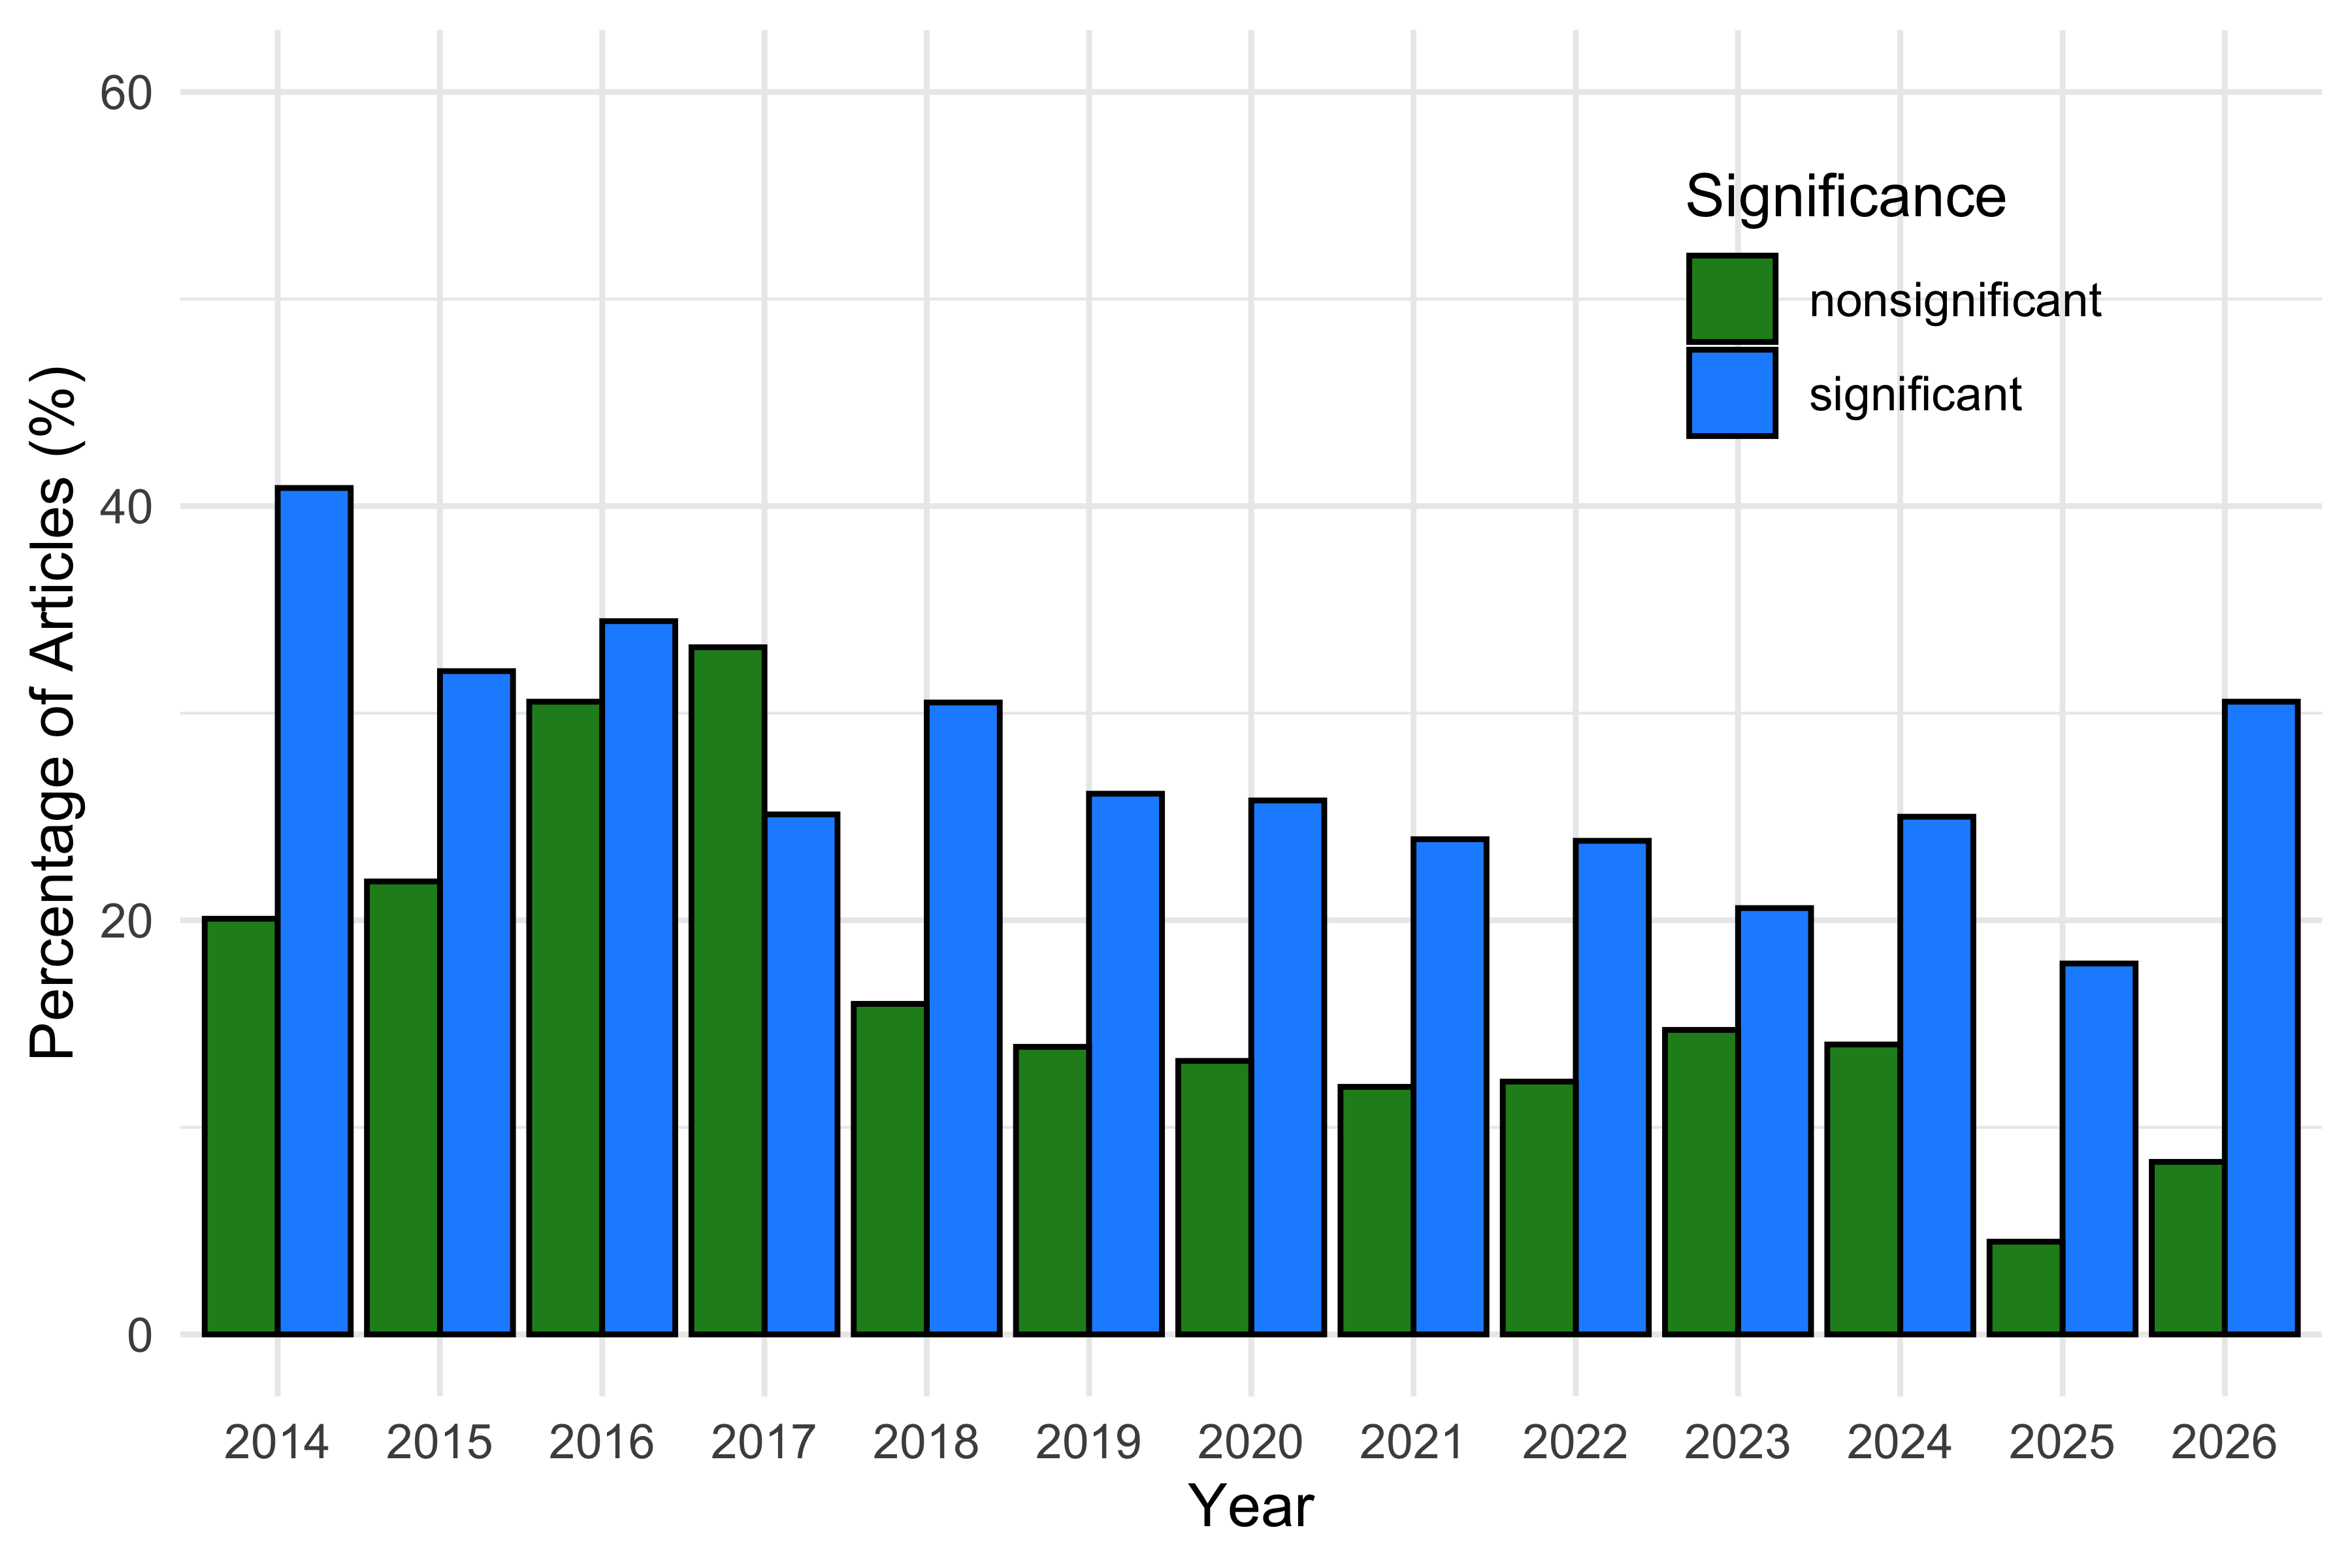
\includegraphics[keepaspectratio]{output/figures/fig-imprecise-pvalues-1.png}}

\apakeepend{0pt}

\par\endgroup\addvspace{\baselineskip}

\par\addvspace{\baselineskip}\begingroup

\setlength{\parindent}{0pt}

\captionsetup{type=figure}

\apatablekeep

\setcounter{figure}{1}

\refstepcounter{figure}%
\makeatletter\def\@currentlabel{2}\makeatother%
\label{fig-atleastone}

\apafloattitle{Figure 2}

\apafloatcaption{Proportion of articles with at least one imprecisely
reported \emph{p} value.}

\apafigureskip

\addcontentsline{lof}{figure}{Figure 2. Proportion of articles with at
least one imprecisely reported \emph{p} value.}

\pandocbounded{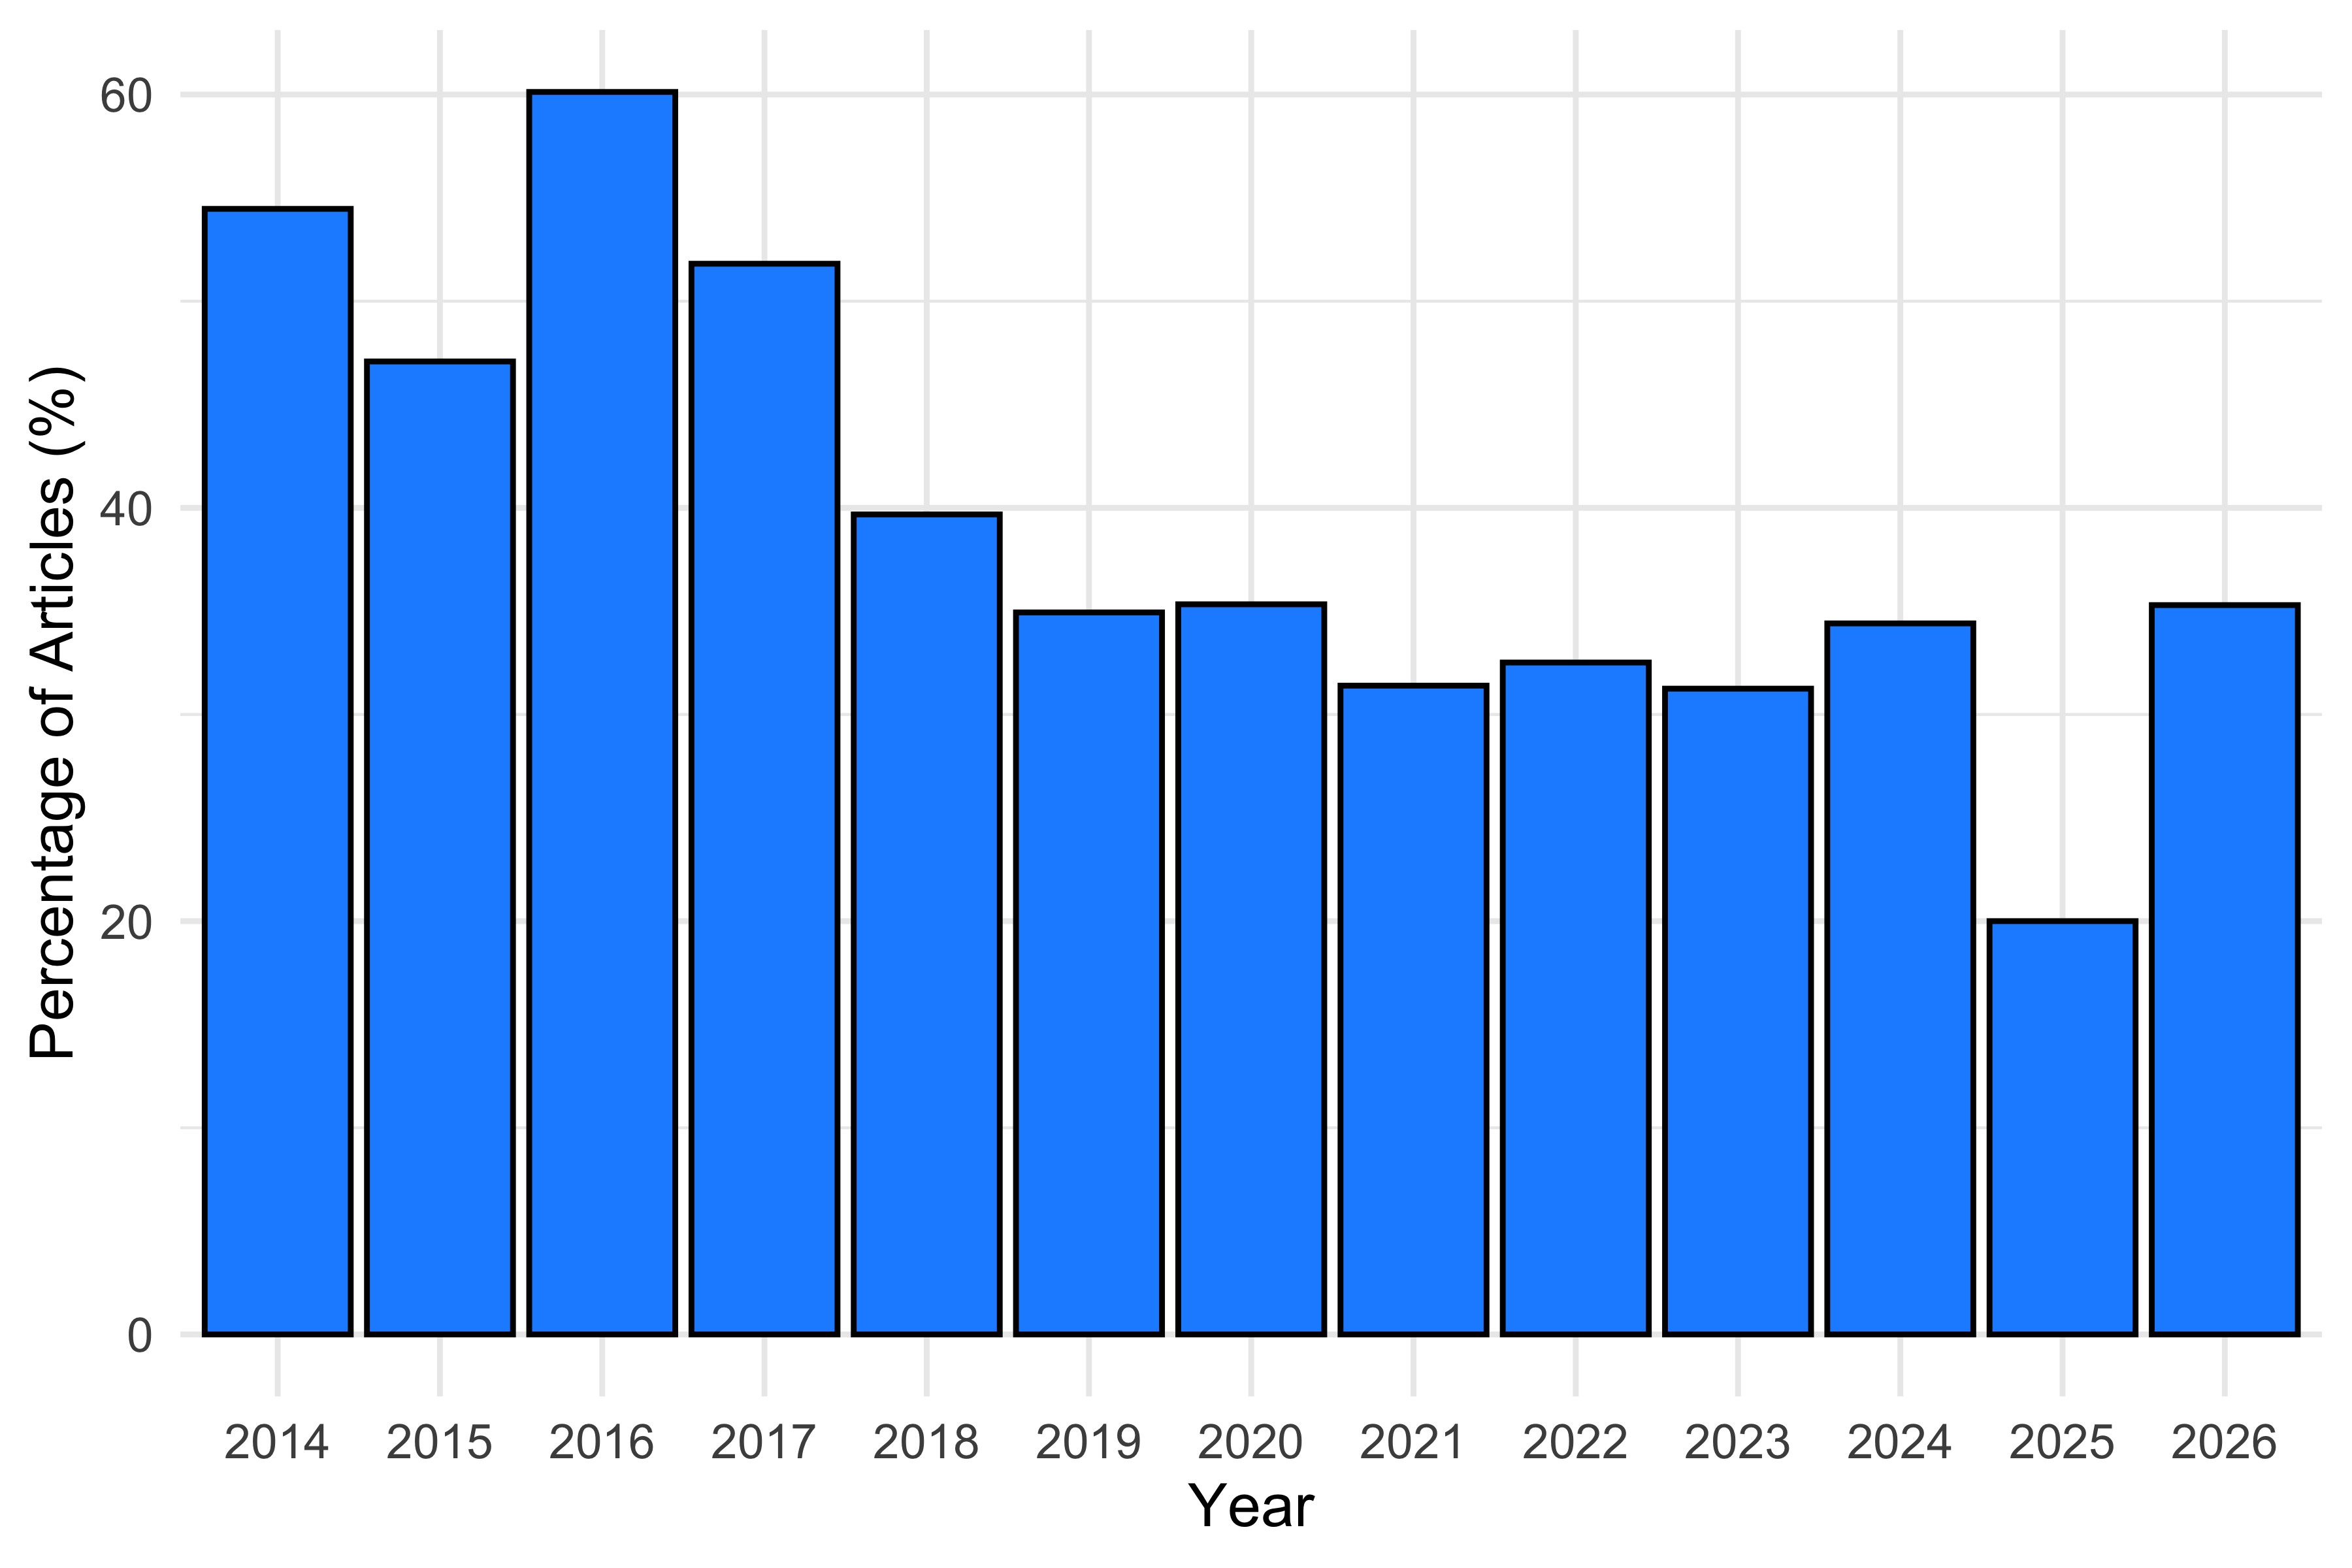
\includegraphics[keepaspectratio]{output/figures/fig-atleastone-1.png}}

\apakeepend{0pt}

\par\endgroup\addvspace{\baselineskip}

The module has also flagged 19 \emph{p} values of .000 across 11
articles, which could have easily been prevented had authors used
Metacheck. Another example is illustrated in
\hyperref[fig-hist]{Figure~\ref*{fig-hist}}, which shows the
distribution of imprecisely reported \emph{p} values by comparator
symbol. This type of overview can reveal interesting exploratory
patterns, such as a large peak around \emph{p} \textgreater{} 0.25. This
may indicate that researchers commonly use 0.25 as a threshold for
interpreting a result as non-significant, although the origin of this
practice is unclear. One possible source is the recommendation to use an
alpha level between 0.25 and 0.35 as a stopping criterion in forward
step-wise selection procedures
(\citeproc{ref-bendel1977comparison}{Bendel \& Afifi, 1977}), which was
later popularized as alpha \(\le\) 0.25 in a widely used textbook on
logistic regression (\citeproc{ref-hosmer2013applied}{Hosmer Jr et al.,
2013}). However, we have no evidence this is the source of the
convention. The correct approach for concluding that an effect is not
meaningful (i.e., equivalent to zero) is to perform an equivalence test
against a smallest effect size of interest
(\citeproc{ref-lakens_equivalence_2018}{Lakens et al., 2018}).

\par\addvspace{\baselineskip}\begingroup

\setlength{\parindent}{0pt}

\captionsetup{type=figure}

\apatablekeep

\setcounter{figure}{2}

\refstepcounter{figure}%
\makeatletter\def\@currentlabel{3}\makeatother%
\label{fig-hist}

\apafloattitle{Figure 3}

\apafloatcaption{Distribution of imprecisely reported \emph{p} values by
comparator}

\apafigureskip

\addcontentsline{lof}{figure}{Figure 3. Distribution of imprecisely
reported \emph{p} values by comparator}

\pandocbounded{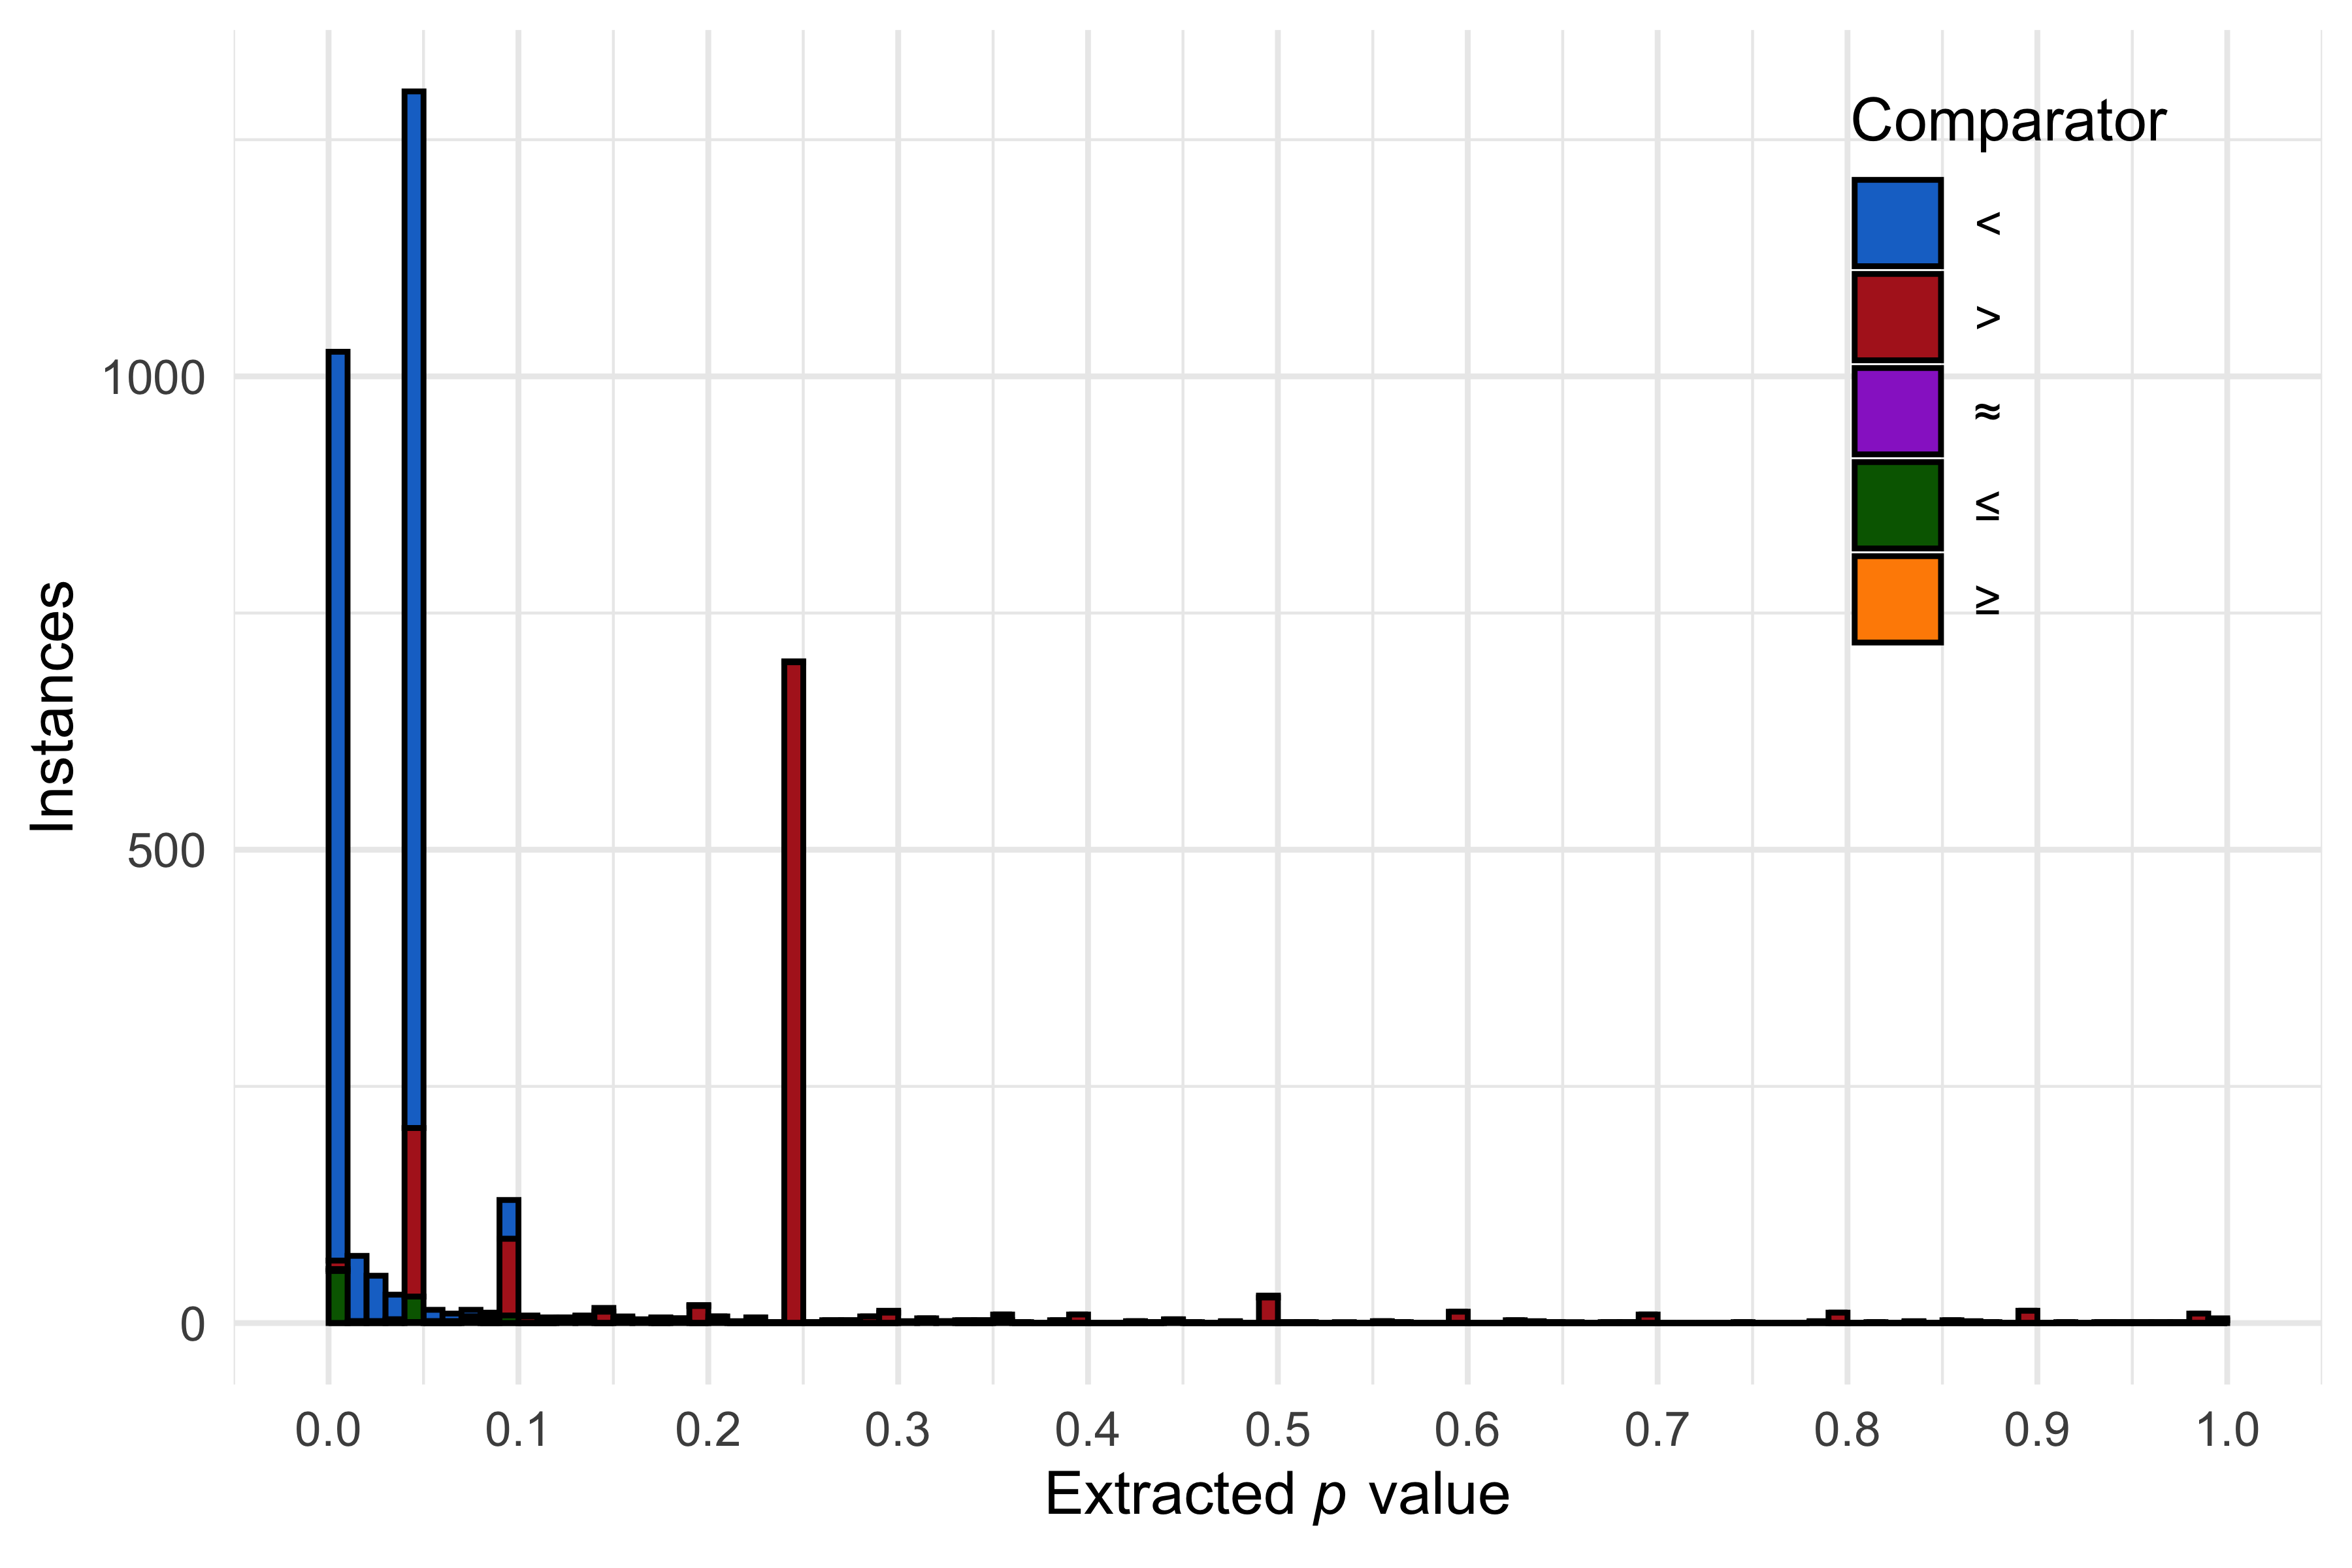
\includegraphics[keepaspectratio]{output/figures/fig-hist-1.png}}

\apakeepend{0pt}

\par\endgroup\addvspace{\baselineskip}

The performance of the \texttt{stat\_p\_exact} module was evaluated on
226 open-access articles published in Psychological Science, for which a
ground-truth dataset was manually created. This set of articles
contained 5019 \emph{p} values, of which 438 were instances of non-exact
\emph{p} values and 4581 instances of exact \emph{p} values. It
correctly detected 420 of 438 instances (96\%) and incorrectly flagged
56 of the 4581 precisely reported \emph{p} values (1.2\%). The module
missed 18 instances (4\%) of imprecisely reported \emph{p} values, and
correctly identified 4525 instances of precisely reported \emph{p}
values.

We have also developed a related module, \texttt{stat\_p\_nonsig} that
detects whether non-significant \emph{p} values are reported in an
article. When such results are identified, the module warns researchers
against the common practice of interpreting non-significant \emph{p}
values as evidence of the absence of an effect and returns all sentences
containing non-significant \emph{p} values, allowing researchers to
quickly check for potential misinterpretations.
\hyperref[tbl-non_sig]{Table~\ref*{tbl-non_sig}} displays the
non-significant \emph{p} value and the full sentence in which it was
reported.

\par\addvspace{\baselineskip}\begingroup

\setlength{\LTleft}{0pt}\setlength{\LTright}{\fill}\setlength{\LTpost}{0pt}\setlength{\apatablenotegap}{-0.5pt}

\setlength{\LTpre}{16pt}

\apatablekeep

\setcounter{table}{1}

\refstepcounter{table}%
\makeatletter\def\@currentlabel{2}\makeatother%
\label{tbl-non_sig}

\apafloattitle{Table 2}

\apafloatcaption{Example output of the \texttt{stat\_p\_nonsig} module
applied to a single article.}

\addcontentsline{lot}{table}{Table 2. Example output of the
\texttt{stat\_p\_nonsig} module applied to a single article.}

\apatablekeepend

\par\ifdim\prevdepth>0pt\vskip-\prevdepth\prevdepth=0pt\fi

\global\setlength{\Oldarrayrulewidth}{\arrayrulewidth}

\global\setlength{\Oldtabcolsep}{\tabcolsep}

\setlength{\tabcolsep}{2pt}

\renewcommand*{\arraystretch}{1.5}



\providecommand{\ascline}[3]{\noalign{\global\arrayrulewidth #1}\arrayrulecolor[HTML]{#2}\cline{#3}}

\begin{longtable*}[c]{|p{1.00in}|p{5.00in}}



\ascline{1.5pt}{666666}{1-2}

\multicolumn{1}{>{\raggedright}m{\dimexpr 1in+0\tabcolsep}}{\textcolor[HTML]{000000}{\fontsize{11}{11}\selectfont{\global\setmainfont{Helvetica}{Text}}}} & \multicolumn{1}{>{\raggedright}m{\dimexpr 5in+0\tabcolsep}}{\textcolor[HTML]{000000}{\fontsize{11}{11}\selectfont{\global\setmainfont{Helvetica}{Expanded}}}} \\

\ascline{1.5pt}{666666}{1-2}\endfirsthead 

\ascline{1.5pt}{666666}{1-2}

\multicolumn{1}{>{\raggedright}m{\dimexpr 1in+0\tabcolsep}}{\textcolor[HTML]{000000}{\fontsize{11}{11}\selectfont{\global\setmainfont{Helvetica}{Text}}}} & \multicolumn{1}{>{\raggedright}m{\dimexpr 5in+0\tabcolsep}}{\textcolor[HTML]{000000}{\fontsize{11}{11}\selectfont{\global\setmainfont{Helvetica}{Expanded}}}} \\

\ascline{1.5pt}{666666}{1-2}\endhead
\endlastfoot



\multicolumn{1}{>{\raggedright}m{\dimexpr 1in+0\tabcolsep}}{\textcolor[HTML]{000000}{\fontsize{11}{11}\selectfont{\global\setmainfont{Helvetica}{p\ =\ .231}}}} & \multicolumn{1}{>{\raggedright}m{\dimexpr 5in+0\tabcolsep}}{\textcolor[HTML]{000000}{\fontsize{11}{11}\selectfont{\global\setmainfont{Helvetica}{Exclusions\ did\ not\ differ\ by\ condition\ (responsive\ questions\ vs.\ unresponsive\ advice),\ b\ =\ -0.04,\ SE\ =\ 0.03,\ t(471)\ =\ -1.20,\ p\ =\ .231,\ p\ adj\ =\ .273.}}}} \\

\ascline{1.5pt}{666666}{1-2}



\end{longtable*}



\arrayrulecolor[HTML]{000000}

\global\setlength{\arrayrulewidth}{\Oldarrayrulewidth}

\global\setlength{\tabcolsep}{\Oldtabcolsep}

\renewcommand*{\arraystretch}{1}

\par\endgroup\addvspace{\baselineskip}

When a non-significant \emph{p} value is detected, the module provides
the following recommendation on how to interpret the a non-significant
result:

\begin{quote}
``Meta-scientific research has shown nonsignificant p values are
commonly misinterpreted. It is incorrect to infer that there is `no
effect', `no difference', or that groups are `the same' after p
\textgreater{} 0.05. It is possible that there is a true non-zero
effect, but that the study did not detect it. Make sure your inference
acknowledges that it is possible that there is a non-zero effect. It is
correct to include the effect is `not significantly' different, although
this just restates that p \textgreater{} 0.05.''
\end{quote}

The module does not attempt to classify whether these statements
containing non-significant sentences were misinterpreted, but authors
interested in automating this step can use the \texttt{llm} function in
Metacheck to send the results to a (local) LLM and retrieve the
inference.

The performance of the \texttt{stat\_p\_nonsig} module was evaluated on
226 open-access articles published in Psychological Science, for which a
ground-truth dataset was manually created. The set contained 5019
\emph{p} values, of which 1529 were non-significant. The module
correctly identified 1496 of the 1529 non-significant \emph{p} values
(98\%) and missed 33. It correctly left 3428 of the 3490 significant
\emph{p} values unflagged (98\%) and incorrectly classified 62
significant \emph{p} values as non-significant. This corresonds top a
false positive rate of 2\%.

\subsubsection{Checking (Un)reported Effect
Sizes}\label{checking-unreported-effect-sizes}

A second JARS guideline that can be checked automatically is whether
effect sizes are reported alongside their statistical test result. Each
statistical test (e.g., \emph{t}-test or \emph{F}-test) should be
accompanied by the corresponding effect size (e.g., Cohen's \emph{d} or
\(\eta_p^2\)). Metacheck includes a dedicated rule-based module,
\texttt{stat\_effect\_size}, that identifies \emph{t}-tests and
\emph{F}-tests for which no effect size is reported and flags these
instances for further inspection.

\hyperref[fig-es-trend]{Figure~\ref*{fig-es-trend}} shows the results of
applying the module to 1937 published articles in Psychological Science
between 2014 and 2026. In 2014, 51\% of \emph{t}-tests and 37\% of
\emph{F}-tests were reported without an accompanying effect size. By
2024, these proportions had declined to 13\% and 16\%, respectively,
suggesting an improvement in reporting practices, although the
proportion for \emph{t}-tests was higher again in 2025 (42\%). Tools
such as Metacheck may help reduce this percentage even further by
identifying missing effect sizes before articles are submitted or
published.

The performance of the module was evaluated on 250 open-access articles
published in Psychological Science, of which 161 reported at least one
\emph{t}-test or \emph{F}-test. The module's extraction of these 1469
tests was manually checked to create a ground-truth dataset. The module
correctly identified 71\% of \emph{t}-tests reported with effect sizes
and 26\% of \emph{t}-tests reported without effect sizes. For
\emph{F}-tests, the corresponding percentages were 81\% and 11\%. This
level of accuracy is sufficient for meta-scientific research, such as
examining changes in adherence to reporting guidelines over time.

\par\addvspace{\baselineskip}\begingroup

\setlength{\parindent}{0pt}

\captionsetup{type=figure}

\apatablekeep

\setcounter{figure}{3}

\refstepcounter{figure}%
\makeatletter\def\@currentlabel{4}\makeatother%
\label{fig-es-trend}

\apafloattitle{Figure 4}

\apafloatcaption{Proportion of articles reporting \emph{t}-tests or
\emph{F}-tests without effect sizes.}

\apafigureskip

\addcontentsline{lof}{figure}{Figure 4. Proportion of articles reporting
\emph{t}-tests or \emph{F}-tests without effect sizes.}

\pandocbounded{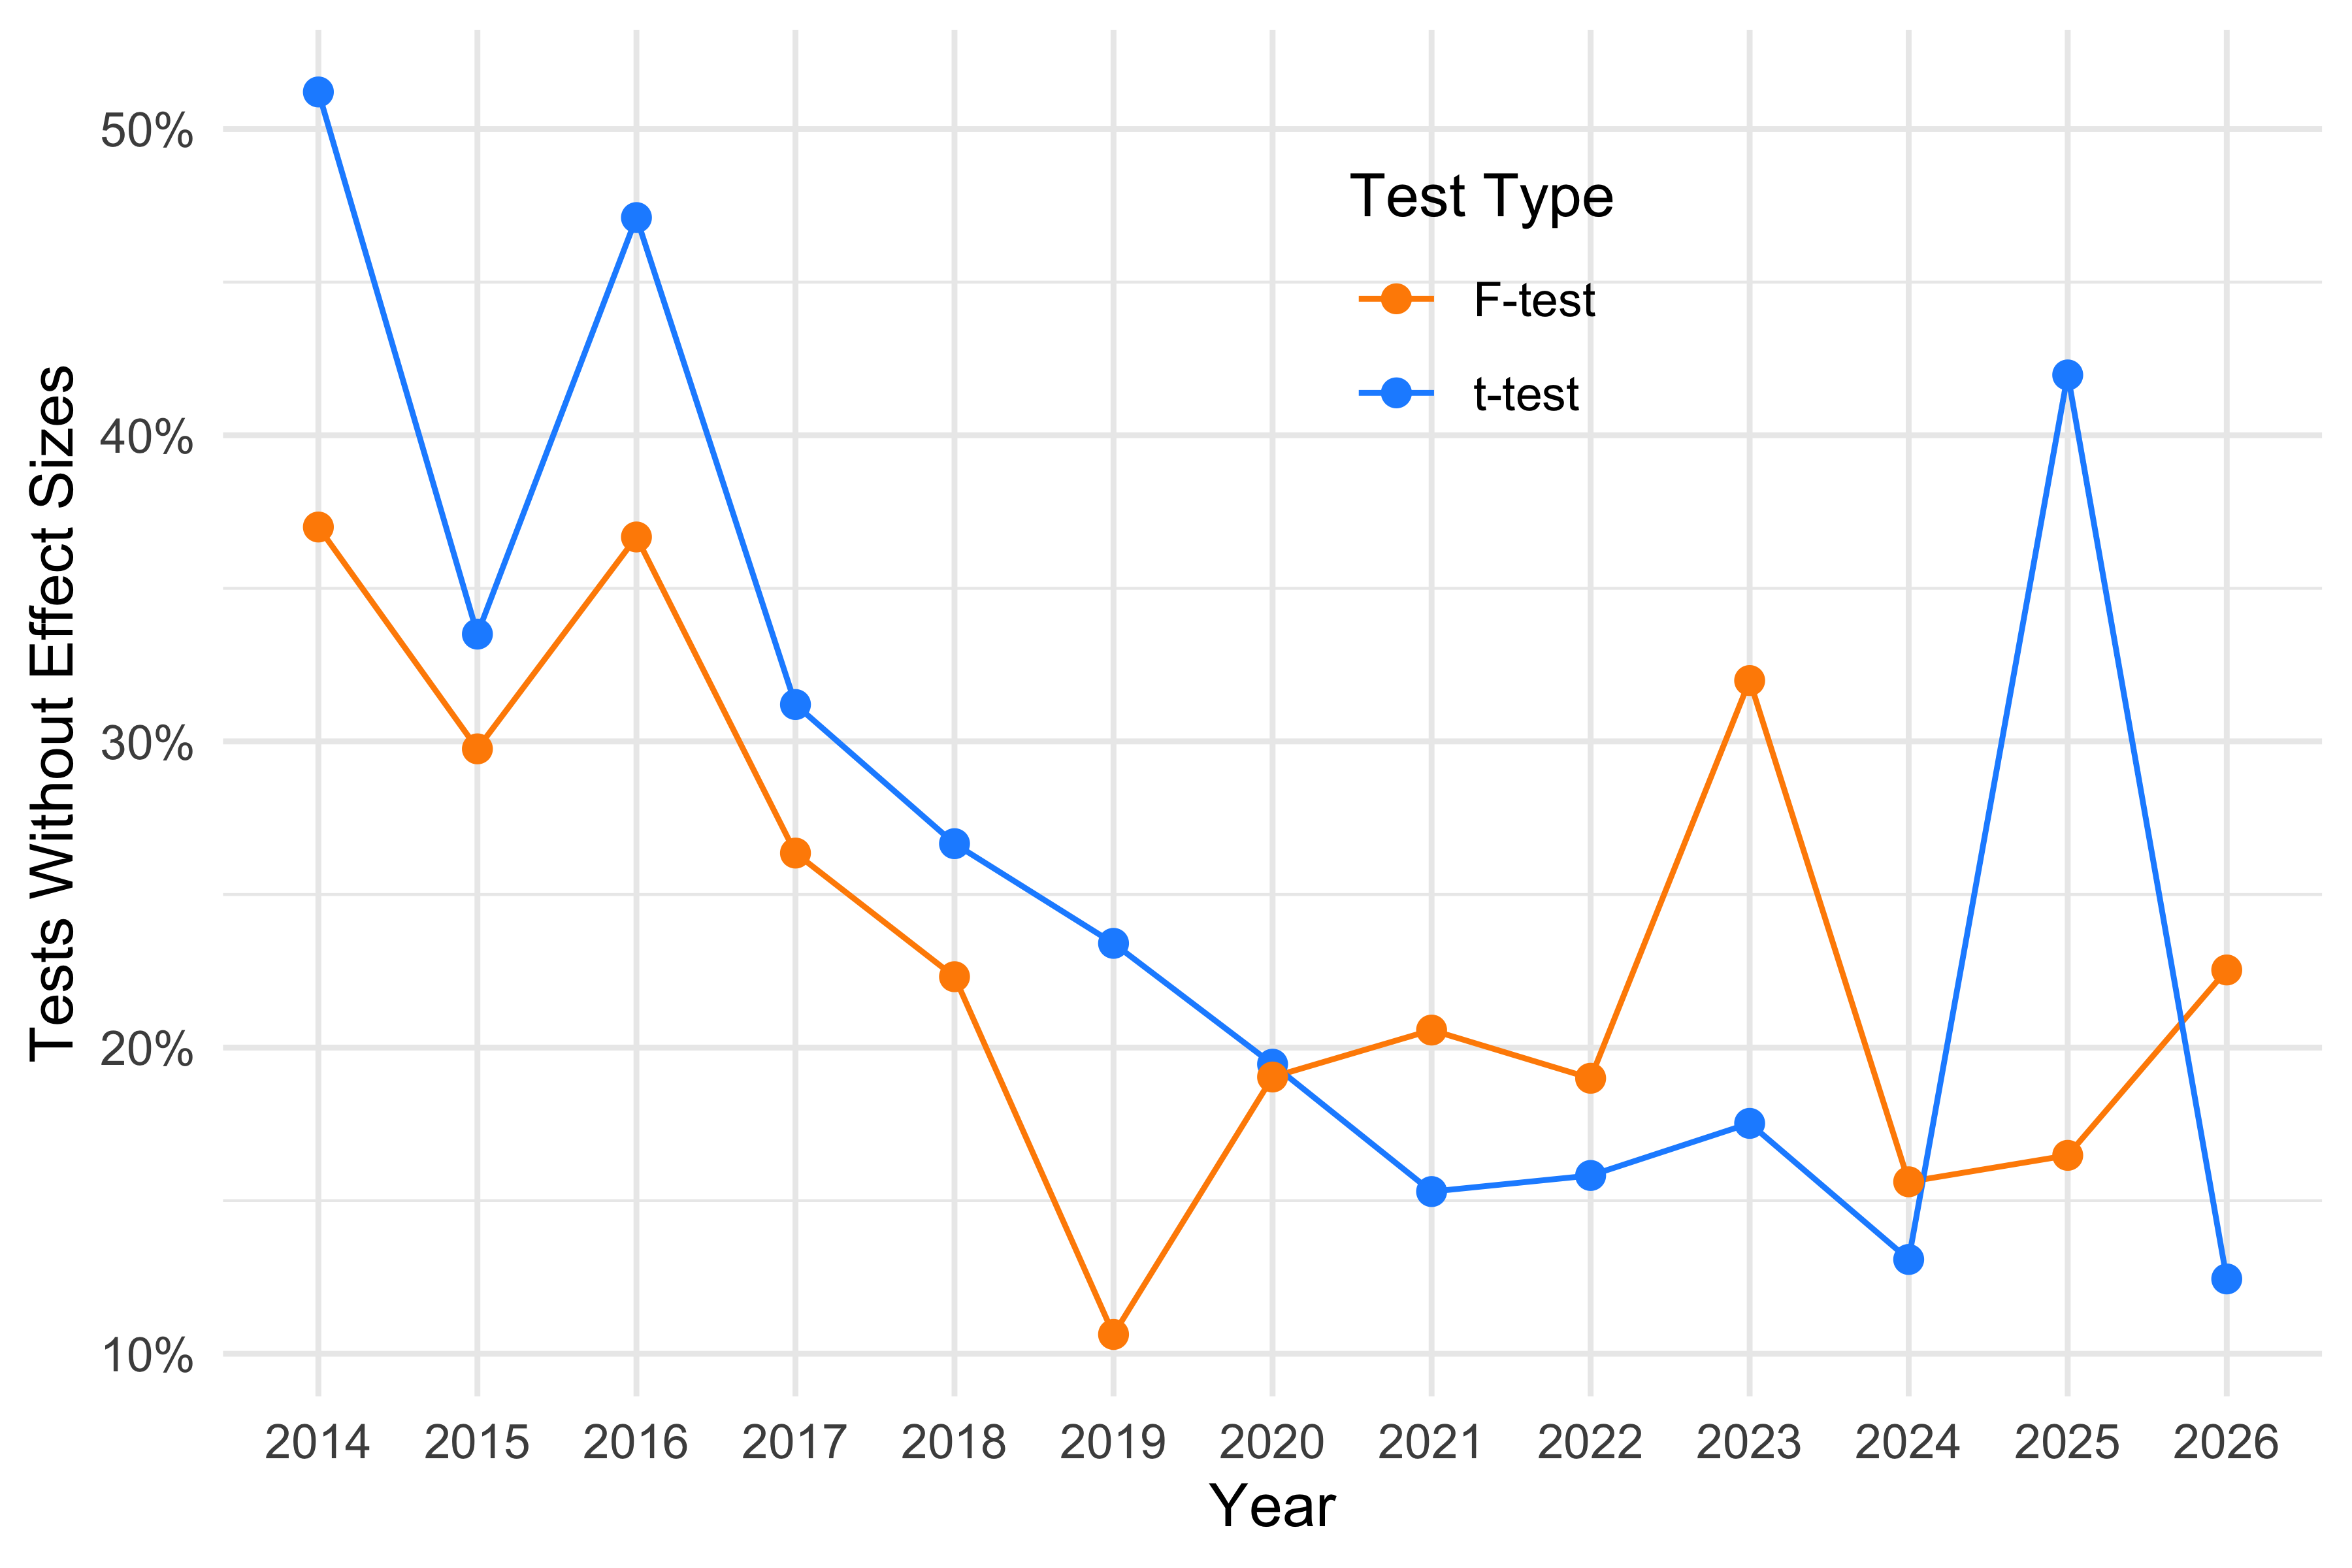
\includegraphics[keepaspectratio]{output/figures/fig-es-trend-1.png}}

\apakeepend{0pt}

\par\endgroup\addvspace{\baselineskip}

Another feature of the \texttt{stat\_effect\_size} is that it checks
whether reported effect sizes are consistent with the corresponding test
statistic and degrees of freedom. For \emph{t}-tests, it checks Cohen's
\emph{d} and Hedges' \emph{g}, while for \emph{F}-tests, it checks
\(\eta_p^2\) and \(\omega_p^2\). Importantly, reporting an effect size
such as \emph{d} = 0.3 does not provide an information about the study
design (i.e., whether the comparison is between or within subjects). The
module therefore computes \emph{d} under several plausible assumptions,
including a Cohen's paired \(d_z\), independent with equal sample sizes,
and a range of possible sample sizes for independent samples. If any of
the recomputed effect sizes matches the reported effect size, the result
is deemed as consistent. \hyperref[tbl-es_d]{Table~\ref*{tbl-es_d}}
displays some of the information returned by the module when checking
the consistency of effect sizes in a single article. The first example
shows a reported effect size that does not match the value implied by
the \emph{t}-test under any of the tested assumptions, whereas the
second is consistent with an independent-samples \emph{t}-test assuming
equal sample sizes.

\par\addvspace{\baselineskip}\begingroup

\setlength{\LTleft}{0pt}\setlength{\LTright}{\fill}\setlength{\LTpost}{0pt}\setlength{\apatablenotegap}{-0.5pt}

\setlength{\LTpre}{16pt}

\apatablekeep

\setcounter{table}{2}

\refstepcounter{table}%
\makeatletter\def\@currentlabel{3}\makeatother%
\label{tbl-es_d}

\apafloattitle{Table 3}

\apafloatcaption{Example output of \texttt{stat\_effect\_size} when
checking the consistency of reported effect sizes with the corresponding
test statistic and degrees of freedom.}

\addcontentsline{lot}{table}{Table 3. Example output of
\texttt{stat\_effect\_size} when checking the consistency of reported
effect sizes with the corresponding test statistic and degrees of
freedom.}

\apatablekeepend

\par\ifdim\prevdepth>0pt\vskip-\prevdepth\prevdepth=0pt\fi

\global\setlength{\Oldarrayrulewidth}{\arrayrulewidth}

\global\setlength{\Oldtabcolsep}{\tabcolsep}

\setlength{\tabcolsep}{2pt}

\renewcommand*{\arraystretch}{1.5}



\providecommand{\ascline}[3]{\noalign{\global\arrayrulewidth #1}\arrayrulecolor[HTML]{#2}\cline{#3}}

\begin{longtable*}[c]{|p{1.00in}|p{1.30in}|p{4.00in}}



\ascline{1.5pt}{666666}{1-3}

\multicolumn{1}{>{\raggedright}m{\dimexpr 1in+0\tabcolsep}}{\textcolor[HTML]{000000}{\fontsize{11}{11}\selectfont{\global\setmainfont{Helvetica}{Text}}}} & \multicolumn{1}{>{\raggedright}m{\dimexpr 1.3in+0\tabcolsep}}{\textcolor[HTML]{000000}{\fontsize{11}{11}\selectfont{\global\setmainfont{Helvetica}{Effect\ Size}}}} & \multicolumn{1}{>{\raggedright}m{\dimexpr 4in+0\tabcolsep}}{\textcolor[HTML]{000000}{\fontsize{11}{11}\selectfont{\global\setmainfont{Helvetica}{Note}}}} \\

\ascline{1.5pt}{666666}{1-3}\endfirsthead 

\ascline{1.5pt}{666666}{1-3}

\multicolumn{1}{>{\raggedright}m{\dimexpr 1in+0\tabcolsep}}{\textcolor[HTML]{000000}{\fontsize{11}{11}\selectfont{\global\setmainfont{Helvetica}{Text}}}} & \multicolumn{1}{>{\raggedright}m{\dimexpr 1.3in+0\tabcolsep}}{\textcolor[HTML]{000000}{\fontsize{11}{11}\selectfont{\global\setmainfont{Helvetica}{Effect\ Size}}}} & \multicolumn{1}{>{\raggedright}m{\dimexpr 4in+0\tabcolsep}}{\textcolor[HTML]{000000}{\fontsize{11}{11}\selectfont{\global\setmainfont{Helvetica}{Note}}}} \\

\ascline{1.5pt}{666666}{1-3}\endhead
\endlastfoot



\multicolumn{1}{>{\raggedright}m{\dimexpr 1in+0\tabcolsep}}{\textcolor[HTML]{000000}{\fontsize{11}{11}\selectfont{\global\setmainfont{Helvetica}{t(169)\ =\ 1.01}}}} & \multicolumn{1}{>{\raggedright}m{\dimexpr 1.3in+0\tabcolsep}}{\textcolor[HTML]{000000}{\fontsize{11}{11}\selectfont{\global\setmainfont{Helvetica}{Cohen's\ d\ =\ 1.38}}}} & \multicolumn{1}{>{\raggedright}m{\dimexpr 4in+0\tabcolsep}}{\textcolor[HTML]{000000}{\fontsize{11}{11}\selectfont{\global\setmainfont{Helvetica}{No\ match\ under\ tested\ assumptions\ (paired\ dz,\ independent\ equal-n,\ independent\ unequal-n\ range).\ Tolerance\ =\ 0.01.\ A\ no-match\ can\ occur\ when\ fewer\ than\ 2\ decimal\ places\ are\ reported.}}}} \\





\multicolumn{1}{>{\raggedright}m{\dimexpr 1in+0\tabcolsep}}{\textcolor[HTML]{000000}{\fontsize{11}{11}\selectfont{\global\setmainfont{Helvetica}{t(183)\ =\ 2.63}}}} & \multicolumn{1}{>{\raggedright}m{\dimexpr 1.3in+0\tabcolsep}}{\textcolor[HTML]{000000}{\fontsize{11}{11}\selectfont{\global\setmainfont{Helvetica}{d\ =\ 0.39}}}} & \multicolumn{1}{>{\raggedright}m{\dimexpr 4in+0\tabcolsep}}{\textcolor[HTML]{000000}{\fontsize{11}{11}\selectfont{\global\setmainfont{Helvetica}{Match\ under\ independent-samples\ equal-n\ assumption\ (n1\ =\ n2\ =\ 92.5,\ N\ =\ 185).}}}} \\

\ascline{1.5pt}{666666}{1-3}



\end{longtable*}



\arrayrulecolor[HTML]{000000}

\global\setlength{\arrayrulewidth}{\Oldarrayrulewidth}

\global\setlength{\tabcolsep}{\Oldtabcolsep}

\renewcommand*{\arraystretch}{1}

\par\endgroup\addvspace{\baselineskip}

\subsubsection{Checking Power Analyses}\label{checking-power-analyses}

To design an informative study, researchers should collect a sufficient
number of observations. The collected sample size should be justified
with respect to the study's inferential goal
(\citeproc{ref-lakens_justification_2022}{Lakens, 2022}). One approach
to do this is by performing an a priori power analysis. When such an
analysis is performed, it should be reported transparently so that peers
can evaluate it.

A transparent power analysis report includes relevant details about the
statistical test for which it was conducted (e.g., an independent
\emph{t}-test, a within-between interaction in a 2 x 2 ANOVA), the
effect size magnitude and metric (e.g., Cohen's \emph{d} = 0.3, \emph{r}
= 0.5, odds ratio = 3.0), the power (e.g., 95\%), sample size, and
critical alpha (e.g., 0.05). The report should also be clear about which
of these values was computed, which is often done using labels like ``a
priori'', ``sensitivity'' or ``post hoc'' (e.g., an a priori analysis
computes sample size, while a sensitivity analysis computes effect
size). The report should also justify the input values (e.g., a smallest
effect size of interest). In practice, however, many articles omit one
or more of these elements, making it difficult to evaluate the power
analysis. In addition, some researchers perform post hoc power analyses
based on the observed effect size and collected sample size, even though
this practice is widely recognized as uninformative and should be
avoided (\citeproc{ref-hoenig_2001}{Hoenig \& Heisey, 2001}).

The \texttt{power} module is designed to help researchers report power
analyses more completely while discouraging the use of post-hoc power
analyses. It can be used with or without LLM's. Without LLM's the module
relies on regular expressions to identify paragraphs that contain the
standalone word \emph{power} (or \emph{powers}/\emph{powered}), at least
one term associated with power analyses (e.g., \emph{effect size},
\emph{sample size}, \emph{a priori}, \emph{sensitivity}, or \emph{post
hoc}), and at least one numeric value, excluding four-digit numbers that
are likely to represent publication years. Because this approach relies
on regular expressions, only power analyses that explicitly contain
terms such as ``a priori'', ``sensitivity'' or ``post hoc'' can be
classified. This use of the module is limited to the classification of
power analyses and does not extract the reported components (e.g.,
effect size metric, statistical test).

A limitation of currently reported power analyses is that they lack a
common reporting standard (e.g., similar to how the APA manual
standardized the reporting of statistical tests). This lack of
standardization makes it difficult, if not impossible, to reliably
extract relevant information from sentences describing a power analysis
using a rule-based approach alone. However, this limitation can be
partially addressed by using an LLM to classify and extract information
from reported power analyses. Based on a predefined prompt, the LLM
returns a structured output containing the identified power analysis
components.

\hyperref[tbl-power_llm]{Table~\ref*{tbl-power_llm}} reports the cases
and proportion of components identified in a sample of 1937 articles. To
generate these results, the \texttt{power} module was run using the
locally hosted Ollama model qwen3.5:9b.

\par\addvspace{\baselineskip}\begingroup

\setlength{\LTleft}{0pt}\setlength{\LTright}{\fill}\setlength{\LTpost}{0pt}\setlength{\apatablenotegap}{-0.5pt}

\setlength{\LTpre}{16pt}

\apatablekeep

\setcounter{table}{3}

\refstepcounter{table}%
\makeatletter\def\@currentlabel{4}\makeatother%
\label{tbl-power_llm}

\apafloattitle{Table 4}

\apafloatcaption{Proportion of missing components from 1295 power
analyses.}

\addcontentsline{lot}{table}{Table 4. Proportion of missing components
from 1295 power analyses.}

\apatablekeepend

\par\ifdim\prevdepth>0pt\vskip-\prevdepth\prevdepth=0pt\fi

\global\setlength{\Oldarrayrulewidth}{\arrayrulewidth}

\global\setlength{\Oldtabcolsep}{\tabcolsep}

\setlength{\tabcolsep}{2pt}

\renewcommand*{\arraystretch}{1.5}



\providecommand{\ascline}[3]{\noalign{\global\arrayrulewidth #1}\arrayrulecolor[HTML]{#2}\cline{#3}}

\begin{longtable*}[c]{|p{2.00in}|p{1.00in}|p{1.00in}}



\ascline{1.5pt}{666666}{1-3}

\multicolumn{1}{>{\raggedright}m{\dimexpr 2in+0\tabcolsep}}{\textcolor[HTML]{000000}{\fontsize{11}{11}\selectfont{\global\setmainfont{Helvetica}{Component}}}} & \multicolumn{1}{>{\raggedleft}m{\dimexpr 1in+0\tabcolsep}}{\textcolor[HTML]{000000}{\fontsize{11}{11}\selectfont{\global\setmainfont{Helvetica}{Missing}}}} & \multicolumn{1}{>{\raggedleft}m{\dimexpr 1in+0\tabcolsep}}{\textcolor[HTML]{000000}{\fontsize{11}{11}\selectfont{\global\setmainfont{Helvetica}{Percent}}}} \\

\ascline{1.5pt}{666666}{1-3}\endfirsthead 

\ascline{1.5pt}{666666}{1-3}

\multicolumn{1}{>{\raggedright}m{\dimexpr 2in+0\tabcolsep}}{\textcolor[HTML]{000000}{\fontsize{11}{11}\selectfont{\global\setmainfont{Helvetica}{Component}}}} & \multicolumn{1}{>{\raggedleft}m{\dimexpr 1in+0\tabcolsep}}{\textcolor[HTML]{000000}{\fontsize{11}{11}\selectfont{\global\setmainfont{Helvetica}{Missing}}}} & \multicolumn{1}{>{\raggedleft}m{\dimexpr 1in+0\tabcolsep}}{\textcolor[HTML]{000000}{\fontsize{11}{11}\selectfont{\global\setmainfont{Helvetica}{Percent}}}} \\

\ascline{1.5pt}{666666}{1-3}\endhead
\endlastfoot



\multicolumn{1}{>{\raggedright}m{\dimexpr 2in+0\tabcolsep}}{\textcolor[HTML]{000000}{\fontsize{11}{11}\selectfont{\global\setmainfont{Helvetica}{power\ type}}}} & \multicolumn{1}{>{\raggedleft}m{\dimexpr 1in+0\tabcolsep}}{\textcolor[HTML]{000000}{\fontsize{11}{11}\selectfont{\global\setmainfont{Helvetica}{0}}}} & \multicolumn{1}{>{\raggedleft}m{\dimexpr 1in+0\tabcolsep}}{\textcolor[HTML]{000000}{\fontsize{11}{11}\selectfont{\global\setmainfont{Helvetica}{0\%}}}} \\





\multicolumn{1}{>{\raggedright}m{\dimexpr 2in+0\tabcolsep}}{\textcolor[HTML]{000000}{\fontsize{11}{11}\selectfont{\global\setmainfont{Helvetica}{power}}}} & \multicolumn{1}{>{\raggedleft}m{\dimexpr 1in+0\tabcolsep}}{\textcolor[HTML]{000000}{\fontsize{11}{11}\selectfont{\global\setmainfont{Helvetica}{199}}}} & \multicolumn{1}{>{\raggedleft}m{\dimexpr 1in+0\tabcolsep}}{\textcolor[HTML]{000000}{\fontsize{11}{11}\selectfont{\global\setmainfont{Helvetica}{15\%}}}} \\





\multicolumn{1}{>{\raggedright}m{\dimexpr 2in+0\tabcolsep}}{\textcolor[HTML]{000000}{\fontsize{11}{11}\selectfont{\global\setmainfont{Helvetica}{sample\ size}}}} & \multicolumn{1}{>{\raggedleft}m{\dimexpr 1in+0\tabcolsep}}{\textcolor[HTML]{000000}{\fontsize{11}{11}\selectfont{\global\setmainfont{Helvetica}{240}}}} & \multicolumn{1}{>{\raggedleft}m{\dimexpr 1in+0\tabcolsep}}{\textcolor[HTML]{000000}{\fontsize{11}{11}\selectfont{\global\setmainfont{Helvetica}{19\%}}}} \\





\multicolumn{1}{>{\raggedright}m{\dimexpr 2in+0\tabcolsep}}{\textcolor[HTML]{000000}{\fontsize{11}{11}\selectfont{\global\setmainfont{Helvetica}{effect\ size}}}} & \multicolumn{1}{>{\raggedleft}m{\dimexpr 1in+0\tabcolsep}}{\textcolor[HTML]{000000}{\fontsize{11}{11}\selectfont{\global\setmainfont{Helvetica}{420}}}} & \multicolumn{1}{>{\raggedleft}m{\dimexpr 1in+0\tabcolsep}}{\textcolor[HTML]{000000}{\fontsize{11}{11}\selectfont{\global\setmainfont{Helvetica}{32\%}}}} \\





\multicolumn{1}{>{\raggedright}m{\dimexpr 2in+0\tabcolsep}}{\textcolor[HTML]{000000}{\fontsize{11}{11}\selectfont{\global\setmainfont{Helvetica}{effect\ size\ metric}}}} & \multicolumn{1}{>{\raggedleft}m{\dimexpr 1in+0\tabcolsep}}{\textcolor[HTML]{000000}{\fontsize{11}{11}\selectfont{\global\setmainfont{Helvetica}{361}}}} & \multicolumn{1}{>{\raggedleft}m{\dimexpr 1in+0\tabcolsep}}{\textcolor[HTML]{000000}{\fontsize{11}{11}\selectfont{\global\setmainfont{Helvetica}{28\%}}}} \\





\multicolumn{1}{>{\raggedright}m{\dimexpr 2in+0\tabcolsep}}{\textcolor[HTML]{000000}{\fontsize{11}{11}\selectfont{\global\setmainfont{Helvetica}{alpha\ level}}}} & \multicolumn{1}{>{\raggedleft}m{\dimexpr 1in+0\tabcolsep}}{\textcolor[HTML]{000000}{\fontsize{11}{11}\selectfont{\global\setmainfont{Helvetica}{868}}}} & \multicolumn{1}{>{\raggedleft}m{\dimexpr 1in+0\tabcolsep}}{\textcolor[HTML]{000000}{\fontsize{11}{11}\selectfont{\global\setmainfont{Helvetica}{67\%}}}} \\





\multicolumn{1}{>{\raggedright}m{\dimexpr 2in+0\tabcolsep}}{\textcolor[HTML]{000000}{\fontsize{11}{11}\selectfont{\global\setmainfont{Helvetica}{statistical\ test}}}} & \multicolumn{1}{>{\raggedleft}m{\dimexpr 1in+0\tabcolsep}}{\textcolor[HTML]{000000}{\fontsize{11}{11}\selectfont{\global\setmainfont{Helvetica}{279}}}} & \multicolumn{1}{>{\raggedleft}m{\dimexpr 1in+0\tabcolsep}}{\textcolor[HTML]{000000}{\fontsize{11}{11}\selectfont{\global\setmainfont{Helvetica}{22\%}}}} \\





\multicolumn{1}{>{\raggedright}m{\dimexpr 2in+0\tabcolsep}}{\textcolor[HTML]{000000}{\fontsize{11}{11}\selectfont{\global\setmainfont{Helvetica}{software}}}} & \multicolumn{1}{>{\raggedleft}m{\dimexpr 1in+0\tabcolsep}}{\textcolor[HTML]{000000}{\fontsize{11}{11}\selectfont{\global\setmainfont{Helvetica}{920}}}} & \multicolumn{1}{>{\raggedleft}m{\dimexpr 1in+0\tabcolsep}}{\textcolor[HTML]{000000}{\fontsize{11}{11}\selectfont{\global\setmainfont{Helvetica}{71\%}}}} \\

\ascline{1.5pt}{666666}{1-3}



\end{longtable*}



\arrayrulecolor[HTML]{000000}

\global\setlength{\arrayrulewidth}{\Oldarrayrulewidth}

\global\setlength{\tabcolsep}{\Oldtabcolsep}

\renewcommand*{\arraystretch}{1}

\par\endgroup\addvspace{\baselineskip}

\textbf{Note}. The number of missing cases for `power\_type' is 0
because the LLM classified all instances into a power-analysis category.

For the 1937 articles published in \emph{Psychological Science}, the
module using the LLM-based approach currently identifies and extracts
information from 663 articles containing 1295 identified power analyses.
Not all missing information is equally problematic. For example, a
missing alpha level is less concerning because the conventional value of
5\% is used in most studies, although some researchers use more
stringent thresholds (e.g., 0.01) or adjust alpha levels to account for
multiple comparisons. By contrast, missing information about the
statistical test is more concerning given the multiplicity of
statistical tests used in psychology articles. Missing the expected
effect size is also particularly problematic because this component is
central to justifying the planned sample size.

Given the lack of standardization in how power analyses are reported and
the complexity of human language, false positive and negative errors
should be expected. For an example, the sentence ``Null of 33\% power
Note: The observed p-curve includes 29 statistically significant
(\emph{p} \textless{} .05) results, of which 14 are \emph{p} \textless{}
.025. There were 8 additional results entered but excluded from p-curve
because they were \emph{p} \textgreater{} .05.'' was incorrectly
classified as a sentence describing a power analysis (i.e., a false
positive) due to the presence of a significance level threshold, and
numbers of entities included and excluded in the analysis.

The following sentence is an example of a false negative error: ``We
attempted to recruit 200 participants to have sufficient power to detect
a small to moderate effect size, but in recruiting groups of friends on
campus, we ended up with 199 fluent English speakers (105 female)''.
This statement provides too little information about the details of the
power analysis to be classified as one.

The validation metrics for each component of the power analysis
extracted by the power module using the LLM-based approach are reported
in \hyperref[tbl-power_validation]{Table~\ref*{tbl-power_validation}}.
Of the 224 observed extraction rows and 225 ground-truth rows, 207 were
successfully matched, meaning that an observed extraction could be
aligned with a corresponding ground-truth row. This resulted in 17
unmatched observed rows and 18 unmatched ground-truth rows.

\par\addvspace{\baselineskip}\begingroup

\setlength{\LTleft}{0pt}\setlength{\LTright}{\fill}\setlength{\LTpost}{0pt}\setlength{\apatablenotegap}{-0.5pt}

\setlength{\LTpre}{16pt}

\apatablekeep

\setcounter{table}{4}

\refstepcounter{table}%
\makeatletter\def\@currentlabel{5}\makeatother%
\label{tbl-power_validation}

\apafloattitle{Table 5}

\apafloatcaption{Percentage of matched components for which the observed
and ground-truth values agree.}

\addcontentsline{lot}{table}{Table 5. Percentage of matched components
for which the observed and ground-truth values agree.}

\apatablekeepend

\par\ifdim\prevdepth>0pt\vskip-\prevdepth\prevdepth=0pt\fi

\global\setlength{\Oldarrayrulewidth}{\arrayrulewidth}

\global\setlength{\Oldtabcolsep}{\tabcolsep}

\setlength{\tabcolsep}{2pt}

\renewcommand*{\arraystretch}{1.5}



\providecommand{\ascline}[3]{\noalign{\global\arrayrulewidth #1}\arrayrulecolor[HTML]{#2}\cline{#3}}

\begin{longtable*}[c]{|p{2.00in}|p{1.00in}|p{1.00in}}



\ascline{1.5pt}{666666}{1-3}

\multicolumn{1}{>{\raggedright}m{\dimexpr 2in+0\tabcolsep}}{\textcolor[HTML]{000000}{\fontsize{11}{11}\selectfont{\global\setmainfont{Helvetica}{Component}}}} & \multicolumn{1}{>{\raggedleft}m{\dimexpr 1in+0\tabcolsep}}{\textcolor[HTML]{000000}{\fontsize{11}{11}\selectfont{\global\setmainfont{Helvetica}{Agree\ (n)}}}} & \multicolumn{1}{>{\raggedleft}m{\dimexpr 1in+0\tabcolsep}}{\textcolor[HTML]{000000}{\fontsize{11}{11}\selectfont{\global\setmainfont{Helvetica}{Accuracy}}}} \\

\ascline{1.5pt}{666666}{1-3}\endfirsthead 

\ascline{1.5pt}{666666}{1-3}

\multicolumn{1}{>{\raggedright}m{\dimexpr 2in+0\tabcolsep}}{\textcolor[HTML]{000000}{\fontsize{11}{11}\selectfont{\global\setmainfont{Helvetica}{Component}}}} & \multicolumn{1}{>{\raggedleft}m{\dimexpr 1in+0\tabcolsep}}{\textcolor[HTML]{000000}{\fontsize{11}{11}\selectfont{\global\setmainfont{Helvetica}{Agree\ (n)}}}} & \multicolumn{1}{>{\raggedleft}m{\dimexpr 1in+0\tabcolsep}}{\textcolor[HTML]{000000}{\fontsize{11}{11}\selectfont{\global\setmainfont{Helvetica}{Accuracy}}}} \\

\ascline{1.5pt}{666666}{1-3}\endhead
\endlastfoot



\multicolumn{1}{>{\raggedright}m{\dimexpr 2in+0\tabcolsep}}{\textcolor[HTML]{000000}{\fontsize{11}{11}\selectfont{\global\setmainfont{Helvetica}{power\ type}}}} & \multicolumn{1}{>{\raggedleft}m{\dimexpr 1in+0\tabcolsep}}{\textcolor[HTML]{000000}{\fontsize{11}{11}\selectfont{\global\setmainfont{Helvetica}{165}}}} & \multicolumn{1}{>{\raggedleft}m{\dimexpr 1in+0\tabcolsep}}{\textcolor[HTML]{000000}{\fontsize{11}{11}\selectfont{\global\setmainfont{Helvetica}{80\%}}}} \\





\multicolumn{1}{>{\raggedright}m{\dimexpr 2in+0\tabcolsep}}{\textcolor[HTML]{000000}{\fontsize{11}{11}\selectfont{\global\setmainfont{Helvetica}{statistical\ test}}}} & \multicolumn{1}{>{\raggedleft}m{\dimexpr 1in+0\tabcolsep}}{\textcolor[HTML]{000000}{\fontsize{11}{11}\selectfont{\global\setmainfont{Helvetica}{159}}}} & \multicolumn{1}{>{\raggedleft}m{\dimexpr 1in+0\tabcolsep}}{\textcolor[HTML]{000000}{\fontsize{11}{11}\selectfont{\global\setmainfont{Helvetica}{77\%}}}} \\





\multicolumn{1}{>{\raggedright}m{\dimexpr 2in+0\tabcolsep}}{\textcolor[HTML]{000000}{\fontsize{11}{11}\selectfont{\global\setmainfont{Helvetica}{sample\ size}}}} & \multicolumn{1}{>{\raggedleft}m{\dimexpr 1in+0\tabcolsep}}{\textcolor[HTML]{000000}{\fontsize{11}{11}\selectfont{\global\setmainfont{Helvetica}{173}}}} & \multicolumn{1}{>{\raggedleft}m{\dimexpr 1in+0\tabcolsep}}{\textcolor[HTML]{000000}{\fontsize{11}{11}\selectfont{\global\setmainfont{Helvetica}{84\%}}}} \\





\multicolumn{1}{>{\raggedright}m{\dimexpr 2in+0\tabcolsep}}{\textcolor[HTML]{000000}{\fontsize{11}{11}\selectfont{\global\setmainfont{Helvetica}{alpha\ level}}}} & \multicolumn{1}{>{\raggedleft}m{\dimexpr 1in+0\tabcolsep}}{\textcolor[HTML]{000000}{\fontsize{11}{11}\selectfont{\global\setmainfont{Helvetica}{201}}}} & \multicolumn{1}{>{\raggedleft}m{\dimexpr 1in+0\tabcolsep}}{\textcolor[HTML]{000000}{\fontsize{11}{11}\selectfont{\global\setmainfont{Helvetica}{97\%}}}} \\





\multicolumn{1}{>{\raggedright}m{\dimexpr 2in+0\tabcolsep}}{\textcolor[HTML]{000000}{\fontsize{11}{11}\selectfont{\global\setmainfont{Helvetica}{power}}}} & \multicolumn{1}{>{\raggedleft}m{\dimexpr 1in+0\tabcolsep}}{\textcolor[HTML]{000000}{\fontsize{11}{11}\selectfont{\global\setmainfont{Helvetica}{194}}}} & \multicolumn{1}{>{\raggedleft}m{\dimexpr 1in+0\tabcolsep}}{\textcolor[HTML]{000000}{\fontsize{11}{11}\selectfont{\global\setmainfont{Helvetica}{94\%}}}} \\





\multicolumn{1}{>{\raggedright}m{\dimexpr 2in+0\tabcolsep}}{\textcolor[HTML]{000000}{\fontsize{11}{11}\selectfont{\global\setmainfont{Helvetica}{effect\ size\ metric}}}} & \multicolumn{1}{>{\raggedleft}m{\dimexpr 1in+0\tabcolsep}}{\textcolor[HTML]{000000}{\fontsize{11}{11}\selectfont{\global\setmainfont{Helvetica}{193}}}} & \multicolumn{1}{>{\raggedleft}m{\dimexpr 1in+0\tabcolsep}}{\textcolor[HTML]{000000}{\fontsize{11}{11}\selectfont{\global\setmainfont{Helvetica}{93\%}}}} \\





\multicolumn{1}{>{\raggedright}m{\dimexpr 2in+0\tabcolsep}}{\textcolor[HTML]{000000}{\fontsize{11}{11}\selectfont{\global\setmainfont{Helvetica}{effect\ size}}}} & \multicolumn{1}{>{\raggedleft}m{\dimexpr 1in+0\tabcolsep}}{\textcolor[HTML]{000000}{\fontsize{11}{11}\selectfont{\global\setmainfont{Helvetica}{189}}}} & \multicolumn{1}{>{\raggedleft}m{\dimexpr 1in+0\tabcolsep}}{\textcolor[HTML]{000000}{\fontsize{11}{11}\selectfont{\global\setmainfont{Helvetica}{91\%}}}} \\





\multicolumn{1}{>{\raggedright}m{\dimexpr 2in+0\tabcolsep}}{\textcolor[HTML]{000000}{\fontsize{11}{11}\selectfont{\global\setmainfont{Helvetica}{software}}}} & \multicolumn{1}{>{\raggedleft}m{\dimexpr 1in+0\tabcolsep}}{\textcolor[HTML]{000000}{\fontsize{11}{11}\selectfont{\global\setmainfont{Helvetica}{192}}}} & \multicolumn{1}{>{\raggedleft}m{\dimexpr 1in+0\tabcolsep}}{\textcolor[HTML]{000000}{\fontsize{11}{11}\selectfont{\global\setmainfont{Helvetica}{93\%}}}} \\

\ascline{1.5pt}{666666}{1-3}



\end{longtable*}



\arrayrulecolor[HTML]{000000}

\global\setlength{\arrayrulewidth}{\Oldarrayrulewidth}

\global\setlength{\tabcolsep}{\Oldtabcolsep}

\renewcommand*{\arraystretch}{1}

\par\endgroup\addvspace{\baselineskip}

\textbf{Note}. Accuracy was calculated as the number of agreements for
each component divided by the number of matched cases (207), multiplied
by 100.

\subsubsection{Checking Statements}\label{checking-statements}

So far, we have focused on modules that capture expertise about
statistical practices. However, another category of checks does not
require any specific expertise but can still benefit from automation.
Although these checks are relatively straightforward, they can easily be
overlooked by researchers and reviewers. Metacheck includes several
modules that check for general statements commonly required by journals.
For example, \texttt{ethics\_check} searchers for statements indicating
that ethical approval was obtained for research involving participants;
\texttt{funding\_check} searchers for funding statements; and
\texttt{coi\_check} searches for conflict-of-interest statements. Below
we illustrate two additional modules, \texttt{open\_practices} and
\texttt{prereg\_check}, which automate checks related to open science
practices and preregistration, respectively.

The \texttt{open\_practices} module searches for statements indicating
that data, code, materials, or preregistration are openly available. It
returns the sentences in which such statements are identified and
classifies, for each type of open practice, whether a corresponding
statement was detected.
\hyperref[tbl-open_practices]{Table~\ref*{tbl-open_practices}} shows the
results of applying the module to a single article. The first statement
indicates that both data and code are available, whereas the second
indicates the availability of code only. The third statement reports
that data, analysis code, and experimental scripts are publicly
available. Therefore, the three statements have been correctly
identified.

\par\addvspace{\baselineskip}\begingroup

\setlength{\LTleft}{0pt}\setlength{\LTright}{\fill}\setlength{\LTpost}{0pt}\setlength{\apatablenotegap}{-0.5pt}

\setlength{\LTpre}{16pt}

\apatablekeep

\setcounter{table}{5}

\refstepcounter{table}%
\makeatletter\def\@currentlabel{6}\makeatother%
\label{tbl-open_practices}

\apafloattitle{Table 6}

\apafloatcaption{Example output of the \texttt{open\_practices} module
applied to one single article.}

\addcontentsline{lot}{table}{Table 6. Example output of the
\texttt{open\_practices} module applied to one single article.}

\apatablekeepend

\par\ifdim\prevdepth>0pt\vskip-\prevdepth\prevdepth=0pt\fi

\global\setlength{\Oldarrayrulewidth}{\arrayrulewidth}

\global\setlength{\Oldtabcolsep}{\tabcolsep}

\setlength{\tabcolsep}{2pt}

\renewcommand*{\arraystretch}{1.5}



\providecommand{\ascline}[3]{\noalign{\global\arrayrulewidth #1}\arrayrulecolor[HTML]{#2}\cline{#3}}

\begin{longtable*}[c]{|p{4.00in}|p{0.50in}|p{0.50in}|p{0.50in}|p{0.50in}}



\ascline{1.5pt}{666666}{1-5}

\multicolumn{1}{>{\raggedright}m{\dimexpr 4in+0\tabcolsep}}{\textcolor[HTML]{000000}{\fontsize{11}{11}\selectfont{\global\setmainfont{Helvetica}{Text}}}} & \multicolumn{1}{>{\raggedleft}m{\dimexpr 0.5in+0\tabcolsep}}{\textcolor[HTML]{000000}{\fontsize{11}{11}\selectfont{\global\setmainfont{Helvetica}{Data}}}} & \multicolumn{1}{>{\raggedleft}m{\dimexpr 0.5in+0\tabcolsep}}{\textcolor[HTML]{000000}{\fontsize{11}{11}\selectfont{\global\setmainfont{Helvetica}{Code}}}} & \multicolumn{1}{>{\raggedleft}m{\dimexpr 0.5in+0\tabcolsep}}{\textcolor[HTML]{000000}{\fontsize{11}{11}\selectfont{\global\setmainfont{Helvetica}{Materials}}}} & \multicolumn{1}{>{\raggedleft}m{\dimexpr 0.5in+0\tabcolsep}}{\textcolor[HTML]{000000}{\fontsize{11}{11}\selectfont{\global\setmainfont{Helvetica}{Preregistration}}}} \\

\ascline{1.5pt}{666666}{1-5}\endfirsthead 

\ascline{1.5pt}{666666}{1-5}

\multicolumn{1}{>{\raggedright}m{\dimexpr 4in+0\tabcolsep}}{\textcolor[HTML]{000000}{\fontsize{11}{11}\selectfont{\global\setmainfont{Helvetica}{Text}}}} & \multicolumn{1}{>{\raggedleft}m{\dimexpr 0.5in+0\tabcolsep}}{\textcolor[HTML]{000000}{\fontsize{11}{11}\selectfont{\global\setmainfont{Helvetica}{Data}}}} & \multicolumn{1}{>{\raggedleft}m{\dimexpr 0.5in+0\tabcolsep}}{\textcolor[HTML]{000000}{\fontsize{11}{11}\selectfont{\global\setmainfont{Helvetica}{Code}}}} & \multicolumn{1}{>{\raggedleft}m{\dimexpr 0.5in+0\tabcolsep}}{\textcolor[HTML]{000000}{\fontsize{11}{11}\selectfont{\global\setmainfont{Helvetica}{Materials}}}} & \multicolumn{1}{>{\raggedleft}m{\dimexpr 0.5in+0\tabcolsep}}{\textcolor[HTML]{000000}{\fontsize{11}{11}\selectfont{\global\setmainfont{Helvetica}{Preregistration}}}} \\

\ascline{1.5pt}{666666}{1-5}\endhead
\endlastfoot



\multicolumn{1}{>{\raggedright}m{\dimexpr 4in+0\tabcolsep}}{\textcolor[HTML]{000000}{\fontsize{11}{11}\selectfont{\global\setmainfont{Helvetica}{Scripts\ to\ run\ the\ experiment,\ analysis\ scripts,\ and\ data\ are\ available\ at\ this\ project's\ Open\ Science\ Framework\ page\ (https://osf.io/tav35/).}}}} & \multicolumn{1}{>{\raggedleft}m{\dimexpr 0.5in+0\tabcolsep}}{\textcolor[HTML]{000000}{\fontsize{11}{11}\selectfont{\global\setmainfont{Helvetica}{true}}}} & \multicolumn{1}{>{\raggedleft}m{\dimexpr 0.5in+0\tabcolsep}}{\textcolor[HTML]{000000}{\fontsize{11}{11}\selectfont{\global\setmainfont{Helvetica}{true}}}} & \multicolumn{1}{>{\raggedleft}m{\dimexpr 0.5in+0\tabcolsep}}{\textcolor[HTML]{000000}{\fontsize{11}{11}\selectfont{\global\setmainfont{Helvetica}{false}}}} & \multicolumn{1}{>{\raggedleft}m{\dimexpr 0.5in+0\tabcolsep}}{\textcolor[HTML]{000000}{\fontsize{11}{11}\selectfont{\global\setmainfont{Helvetica}{false}}}} \\





\multicolumn{1}{>{\raggedright}m{\dimexpr 4in+0\tabcolsep}}{\textcolor[HTML]{000000}{\fontsize{11}{11}\selectfont{\global\setmainfont{Helvetica}{All\ codes\ relevant\ to\ analysis\ of\ the\ main\ and\ supplemental\ findings\ are\ available\ at\ this\ project's\ Open\ Science\ Framework\ page\ (https://osf.io/tav35/).}}}} & \multicolumn{1}{>{\raggedleft}m{\dimexpr 0.5in+0\tabcolsep}}{\textcolor[HTML]{000000}{\fontsize{11}{11}\selectfont{\global\setmainfont{Helvetica}{false}}}} & \multicolumn{1}{>{\raggedleft}m{\dimexpr 0.5in+0\tabcolsep}}{\textcolor[HTML]{000000}{\fontsize{11}{11}\selectfont{\global\setmainfont{Helvetica}{true}}}} & \multicolumn{1}{>{\raggedleft}m{\dimexpr 0.5in+0\tabcolsep}}{\textcolor[HTML]{000000}{\fontsize{11}{11}\selectfont{\global\setmainfont{Helvetica}{false}}}} & \multicolumn{1}{>{\raggedleft}m{\dimexpr 0.5in+0\tabcolsep}}{\textcolor[HTML]{000000}{\fontsize{11}{11}\selectfont{\global\setmainfont{Helvetica}{false}}}} \\





\multicolumn{1}{>{\raggedright}m{\dimexpr 4in+0\tabcolsep}}{\textcolor[HTML]{000000}{\fontsize{11}{11}\selectfont{\global\setmainfont{Helvetica}{All\ data,\ analysis\ code,\ and\ scripts\ to\ run\ the\ experiment\ have\ been\ made\ publicly\ available\ via\ OSF\ and\ can\ be\ accessed\ at\ https://osf.io/tav35/.}}}} & \multicolumn{1}{>{\raggedleft}m{\dimexpr 0.5in+0\tabcolsep}}{\textcolor[HTML]{000000}{\fontsize{11}{11}\selectfont{\global\setmainfont{Helvetica}{true}}}} & \multicolumn{1}{>{\raggedleft}m{\dimexpr 0.5in+0\tabcolsep}}{\textcolor[HTML]{000000}{\fontsize{11}{11}\selectfont{\global\setmainfont{Helvetica}{true}}}} & \multicolumn{1}{>{\raggedleft}m{\dimexpr 0.5in+0\tabcolsep}}{\textcolor[HTML]{000000}{\fontsize{11}{11}\selectfont{\global\setmainfont{Helvetica}{false}}}} & \multicolumn{1}{>{\raggedleft}m{\dimexpr 0.5in+0\tabcolsep}}{\textcolor[HTML]{000000}{\fontsize{11}{11}\selectfont{\global\setmainfont{Helvetica}{false}}}} \\

\ascline{1.5pt}{666666}{1-5}



\end{longtable*}



\arrayrulecolor[HTML]{000000}

\global\setlength{\arrayrulewidth}{\Oldarrayrulewidth}

\global\setlength{\tabcolsep}{\Oldtabcolsep}

\renewcommand*{\arraystretch}{1}

\par\endgroup\addvspace{\baselineskip}

The module also flags statements indicating that data or materials are
available only upon request. For example, in the sample of 1937
articles, the module identified 64 such statements. When an upon-request
statement is detected, the module returns the following warning:

\begin{quote}
Some materials are shared on request, which is not an acceptable method
of sharing. This is based on the following text:
\end{quote}

\begin{quote}
Data for the present experiments are available on request from the
corresponding author.
\end{quote}

Another category of checks that does not require specialised expertise
concerns preregistration. Preregistrations often go unchecked, which is
problematic because studies may deviate from their preregistered plans
without reporting these deviations. Metacheck includes the
\texttt{prereg\_check} module, which identifies links to
preregistrations on OSF and AsPredicted in a manuscript, retrieves their
text, and organises the contents into a standardised template. This
makes it easier for reviewers to compare the preregistered plans with
what is reported in the manuscript and identify potential discrepancies.

To illustrate its use, we show the output of \texttt{prereg\_check}
after running it on a single paper. When the module identifies links to
preregistrations, it returns a summary indicating how many were found.

\begin{quote}
We found 3 preregistrations.
\end{quote}

The module returns a table with one row per preregistrations. The
columns correspond to fields in the standardised preregistration
template. For example, for an OSF preregistration, the table includes
fields such as hypotheses, sample size and statistical tests, among
others.

We can then use the Metacheck's \texttt{text\_search()} function to
extract relevant sentences from the manuscript and compare them with the
corresponding information in the preregistration. For example, we can
search for sentences containing the word ``hypothesis'' and compare the
reported hypotheses with those specified in the preregistration to
identify potential discrepancies. Below we compare the hypothesis
specified in the third preregistration identified above with the
hypothesis reported in the study.

\global\setlength{\Oldarrayrulewidth}{\arrayrulewidth}

\global\setlength{\Oldtabcolsep}{\tabcolsep}

\setlength{\tabcolsep}{2pt}

\renewcommand*{\arraystretch}{1.5}



\providecommand{\ascline}[3]{\noalign{\global\arrayrulewidth #1}\arrayrulecolor[HTML]{#2}\cline{#3}}

\begin{longtable*}[c]{|p{3.15in}|p{3.15in}}



\ascline{1.5pt}{666666}{1-2}

\multicolumn{1}{>{\raggedright}m{\dimexpr 3.15in+0\tabcolsep}}{\textcolor[HTML]{000000}{\fontsize{11}{11}\selectfont{\global\setmainfont{Helvetica}{Preregistration\ hypothesis}}}} & \multicolumn{1}{>{\raggedright}m{\dimexpr 3.15in+0\tabcolsep}}{\textcolor[HTML]{000000}{\fontsize{11}{11}\selectfont{\global\setmainfont{Helvetica}{Study\ hypothesis}}}} \\

\ascline{1.5pt}{666666}{1-2}\endfirsthead 

\ascline{1.5pt}{666666}{1-2}

\multicolumn{1}{>{\raggedright}m{\dimexpr 3.15in+0\tabcolsep}}{\textcolor[HTML]{000000}{\fontsize{11}{11}\selectfont{\global\setmainfont{Helvetica}{Preregistration\ hypothesis}}}} & \multicolumn{1}{>{\raggedright}m{\dimexpr 3.15in+0\tabcolsep}}{\textcolor[HTML]{000000}{\fontsize{11}{11}\selectfont{\global\setmainfont{Helvetica}{Study\ hypothesis}}}} \\

\ascline{1.5pt}{666666}{1-2}\endhead
\endlastfoot



\multicolumn{1}{>{\raggedright}m{\dimexpr 3.15in+0\tabcolsep}}{\textcolor[HTML]{000000}{\fontsize{11}{11}\selectfont{\global\setmainfont{Helvetica}{(H1)\ Adolescents\ in\ the\ motive-alignment\ intervention\ will\ exhibit\ more\ sustainable\ behavior\ compared\ to\ adolescents\ in\ the\ traditional\ environmental\ intervention.\ Sustainable\ behavior\ will\ be\ measured\ in\ terms\ of\ their\ (a)\ food\ choices\ at\ the\ post-intervention\ assessment,\ (b)\ food\ choices\ at\ the\ follow-up\ assessment,\ and\ (c)\ donations\ at\ the\ follow-up\ assessment.}}}} & \multicolumn{1}{>{\raggedright}m{\dimexpr 3.15in+0\tabcolsep}}{\textcolor[HTML]{000000}{\fontsize{11}{11}\selectfont{\global\setmainfont{Helvetica}{Using\ Bayesian\ informative\ hypothesis\ testing,\ we\ evaluated\ the\ hypothesis\ that\ the\ motive-alignment\ intervention\ would\ foster\ more\ proenvironmental\ behavior\ than\ the\ control\ intervention.}}}} \\

\ascline{1.5pt}{666666}{1-2}



\end{longtable*}



\arrayrulecolor[HTML]{000000}

\global\setlength{\arrayrulewidth}{\Oldarrayrulewidth}

\global\setlength{\tabcolsep}{\Oldtabcolsep}

\renewcommand*{\arraystretch}{1}

The same approach can be applied to any preregistration field by
searching the manuscript for relevant terms, such as those related to
sample size or statistical tests. However, this approach requires users
to manually compare the information reported in the manuscript with the
corresponding preregistered information. To facilitate this process, we
have also developed a Metacheck module that sends detected
preregistrations to \href{https://regcheck.app/}{RegCheck}, a fully
automated comparison tool that uses LLMs to compare a manuscript with
its preregistration (\citeproc{ref-cummins_2026}{Cummins et al., 2026}).

\subsubsection{Checking References}\label{checking-references}

Metacheck includes several modules that use an article's references list
of an article to perform automated checks. For example,
\texttt{ref\_retraction} searches for cited articles that have
corrections, expressions of concern, or retractions;
\texttt{ref\_replication} identifies cases in which an original article
is cited but a direct replication study of that article exists and is
not cited, using the Replication Database
(\citeproc{ref-roseler_replication_2024}{{Röseler et al.}, 2024});
\texttt{ref\_accuracy} identifies inconsistencies in references; and
\texttt{ref\_pubpeer} checks whether cited articles have comments on
PubPeer.

For illustrative purposes, we demonstrate the \texttt{ref\_pubpeer}
module, which checks whether references with a DOI have comments on
PubPeer, a platform for post-publication peer review. These comments may
be worth investigating, as they can range from minor clarifications to
serious concerns about the work. The goal is to make this information
more readily available to researchers. Note that a lot of comments on
PubPeer are posted test results from an older version of the Statcheck R
package. We filter these PubPeer comments out because they are generally
uninformative. If the module detects any other comments on a cited
article, it returns the following warning:

\begin{quote}
``We checked 9 references with DOIs. You cited 2 references with
comments in PubPeer. Pubpeer is a platform for post-publication peer
review. We have filtered out Pubpeer comments by Statcheck.
\end{quote}

The module reports which cited articles have comments on PubPeer, the
number of comments, and a link to the corresponding discussion, allowing
users to assess the relevance of each discussion themselves. As
illustrated in \hyperref[tbl-ref_pubpeer]{Table~\ref*{tbl-ref_pubpeer}},
two cited articles have 13 and 2 PubPeer comments respectively, with
links to the corresponding discussions.

\par\addvspace{\baselineskip}\begingroup

\setlength{\LTleft}{0pt}\setlength{\LTright}{\fill}\setlength{\LTpost}{0pt}\setlength{\apatablenotegap}{-0.5pt}

\setlength{\LTpre}{16pt}

\apatablekeep

\setcounter{table}{6}

\refstepcounter{table}%
\makeatletter\def\@currentlabel{7}\makeatother%
\label{tbl-ref_pubpeer}

\apafloattitle{Table 7}

\apafloatcaption{Example output of the \texttt{ref\_pubpeer} module
applied to one single article.}

\addcontentsline{lot}{table}{Table 7. Example output of the
\texttt{ref\_pubpeer} module applied to one single article.}

\apatablekeepend

\par\ifdim\prevdepth>0pt\vskip-\prevdepth\prevdepth=0pt\fi

\global\setlength{\Oldarrayrulewidth}{\arrayrulewidth}

\global\setlength{\Oldtabcolsep}{\tabcolsep}

\setlength{\tabcolsep}{2pt}

\renewcommand*{\arraystretch}{1.5}



\providecommand{\ascline}[3]{\noalign{\global\arrayrulewidth #1}\arrayrulecolor[HTML]{#2}\cline{#3}}

\begin{longtable*}[c]{|p{2.00in}|p{1.00in}|p{4.00in}}



\ascline{1.5pt}{666666}{1-3}

\multicolumn{1}{>{\raggedright}m{\dimexpr 2in+0\tabcolsep}}{\textcolor[HTML]{000000}{\fontsize{11}{11}\selectfont{\global\setmainfont{Helvetica}{DOI}}}} & \multicolumn{1}{>{\raggedleft}m{\dimexpr 1in+0\tabcolsep}}{\textcolor[HTML]{000000}{\fontsize{11}{11}\selectfont{\global\setmainfont{Helvetica}{Comments}}}} & \multicolumn{1}{>{\raggedright}m{\dimexpr 4in+0\tabcolsep}}{\textcolor[HTML]{000000}{\fontsize{11}{11}\selectfont{\global\setmainfont{Helvetica}{URL}}}} \\

\ascline{1.5pt}{666666}{1-3}\endfirsthead 

\ascline{1.5pt}{666666}{1-3}

\multicolumn{1}{>{\raggedright}m{\dimexpr 2in+0\tabcolsep}}{\textcolor[HTML]{000000}{\fontsize{11}{11}\selectfont{\global\setmainfont{Helvetica}{DOI}}}} & \multicolumn{1}{>{\raggedleft}m{\dimexpr 1in+0\tabcolsep}}{\textcolor[HTML]{000000}{\fontsize{11}{11}\selectfont{\global\setmainfont{Helvetica}{Comments}}}} & \multicolumn{1}{>{\raggedright}m{\dimexpr 4in+0\tabcolsep}}{\textcolor[HTML]{000000}{\fontsize{11}{11}\selectfont{\global\setmainfont{Helvetica}{URL}}}} \\

\ascline{1.5pt}{666666}{1-3}\endhead
\endlastfoot



\multicolumn{1}{>{\raggedright}m{\dimexpr 2in+0\tabcolsep}}{\textcolor[HTML]{000000}{\fontsize{11}{11}\selectfont{\global\setmainfont{Helvetica}{10.1177/0956797610383437}}}} & \multicolumn{1}{>{\raggedleft}m{\dimexpr 1in+0\tabcolsep}}{\textcolor[HTML]{000000}{\fontsize{11}{11}\selectfont{\global\setmainfont{Helvetica}{13}}}} & \multicolumn{1}{>{\raggedright}m{\dimexpr 4in+0\tabcolsep}}{\textcolor[HTML]{000000}{\fontsize{11}{11}\selectfont{\global\setmainfont{Helvetica}{https://pubpeer.com/publications/69477CA2ACFC09B9239A8A256F143C}}}} \\





\multicolumn{1}{>{\raggedright}m{\dimexpr 2in+0\tabcolsep}}{\textcolor[HTML]{000000}{\fontsize{11}{11}\selectfont{\global\setmainfont{Helvetica}{10.1177/0956797613492425}}}} & \multicolumn{1}{>{\raggedleft}m{\dimexpr 1in+0\tabcolsep}}{\textcolor[HTML]{000000}{\fontsize{11}{11}\selectfont{\global\setmainfont{Helvetica}{2}}}} & \multicolumn{1}{>{\raggedright}m{\dimexpr 4in+0\tabcolsep}}{\textcolor[HTML]{000000}{\fontsize{11}{11}\selectfont{\global\setmainfont{Helvetica}{https://pubpeer.com/publications/9B511C4BEA5563F50E0BC6DDF1A00B}}}} \\

\ascline{1.5pt}{666666}{1-3}



\end{longtable*}



\arrayrulecolor[HTML]{000000}

\global\setlength{\arrayrulewidth}{\Oldarrayrulewidth}

\global\setlength{\tabcolsep}{\Oldtabcolsep}

\renewcommand*{\arraystretch}{1}

\par\endgroup\addvspace{\baselineskip}

For reference-related modules to work reliably, references must be
accurately extracted from the PDF file, and each reference needs to have
a DOI. However, some journals do not require DOIs in their references,
and older publications may not have one. These limitations make it more
difficult to automate reference-related checks. Metacheck provides two
options to retrieve missing DOIs from CrossRef or OpenAlex. One option
is to set the \texttt{crossref\_lookup\ =\ TRUE} argument in
\texttt{convert()} function, which uses GROBID to convert a PDF file
into XML or JSON format. Alternatively, users can apply
\texttt{add\_bib\_match()} directly to a converted manuscript to
retrieve DOI matches for its references.

\subsection{Validation}\label{validation}

Evaluating the accuracy of automated tools is essential for establishing
their performance. The increasing availability of large language models
(LLMs) has facilitated the development of automated tools, sometimes
with limited direct human involvement in their design and testing. This
makes systematic validation particularly important: How accurately do
these tools perform, and under which circumstances can their outputs be
trusted?

Quality control is one of Metacheck's core values and reflects our
commitment to evaluating the accuracy of its modules through validation.
Ideally, validation should be conducted using datasets that are
representative of the target population of articles to which an
automated tool will be applied. This involves establishing ground truth
and comparing it with the output generated by the automated tool. This
comparison allows instances to be classified as true positives, true
negatives, false positives, and false negatives, from which performance
metrics such as sensitivity, specificity, and positive predictive value
(precision) can be calculated. Because these metrics capture different
aspects of performance, it is important to explicitly report which
metrics are used and how they are calculated.

Equally important is the transparency and reproducibility of the
validation procedure. Documentation should describe how the ground truth
was established, how human judgments were obtained, what constituted a
correct or incorrect extraction, and which data were included in the
evaluation. The limitations of the validation approach should also be
clearly communicated, as these determine the conclusions that can be
drawn about a tool's performance.

For example, the validation of Metacheck's \texttt{stat\_effect\_size}
module involved using the module to identify instances of \emph{t}-tests
and \emph{F}-tests and extract their corresponding effect sizes. The
resulting validation dataset contained the sentences flagged by the
module as reporting these statistical tests, together with the extracted
effect sizes. Human coders subsequently reviewed the detected instances
and classified the module's outputs according to whether an effect size
had been correctly extracted.

An important limitation of this validation approach is that the
validation dataset was constructed using the module itself to identify
statistical tests. Consequently, statistical tests that the module
failed to detect were not included in the dataset and could not be
identified as false negatives. The validation results therefore reflect
the module's accuracy in extracting effect sizes from detected
statistical tests, rather than its overall performance in identifying
all statistical tests and their corresponding effect sizes in an
article. This distinction is important when interpreting the reported
performance metrics.

\begin{verbatim}
Rows: 1469 Columns: 15
-- Column specification --------------------------------------------------------
Delimiter: ","
chr (9): id, text, section, es, test_text, test, notes, es_outcome, test_out...
dbl (3): div, p, s
lgl (3): es_valid, test_text_valid, test_valid

i Use `spec()` to retrieve the full column specification for this data.
i Specify the column types or set `show_col_types = FALSE` to quiet this message.
\end{verbatim}

Furthermore, examining the situations in which false positives and false
negatives occur can help users understand the module's limitations. For
example, our validation suggests that the module failed to recognize 8
regression coefficients reported using the beta symbol (β). It also
missed 5 effect sizes reported using expressions such as ``slope =''.
These examples illustrate how differences in reporting conventions can
affect extraction accuracy and highlight opportunities for improving the
module.

Improving validation practices across Metacheck is an ongoing priority.
We are committed to continuously strengthening our validation
procedures, improving the documentation and transparency of our
evaluations, and ensuring that our modules are assessed using
reproducible workflows. As Metacheck evolves, we will continue to review
and improve our validation practices to increase confidence in the
accuracy of its modules.

\subsection{Creating Metacheck
Modules}\label{creating-metacheck-modules}

Metacheck is modular by design. Its modules are conceptually similar to
functions in R packages: each module performs a specific automated
check, and provides feedback in a structured output format that can be
further analysed or integrated in the reports that can be generated with
Metacheck. This architecture reflects two core values of Metacheck:
community engagement and epistemic diversity. We belive that decisions
about what constitutes best research practice should emerge from
scientific discussions rather than be imposed by a single group.
Accordingly, Metacheck is designed to make it as easy as possible for
researchers to translate their own views on best practices into modules.

Anyone can develop a module and validate its performance. Modules can be
developed and installed locally or contributed to the Metacheck R
package through a GitHub pull request. This flexibility allows journals
to develop modules that verify compliance with their submission
guidelines, methodological experts to automate checks for issues they
frequently encounter during peer review, and organizations to create
modules that assess adherence to their published reporting guidelines.

Through its modular architecture, Metacheck can also serve as a hub for
existing automated tools. An increasing number number of tool developers
are creating useful automated checks. By providing a single entry point
to all available automated checks, Metacheck makes them easier to access
and discover while providing a common infrastructure for PDF import,
file conversion, text searching, and structured output.

As proof of concept, we developed a Metacheck module for Statcheck
(\citeproc{ref-nuijten_2016}{Nuijten et al., 2016}). However, consistent
with Metacheck's emphasis on validated automated checks, the module only
implements check for \emph{t}-tests and \emph{F}-tests. An initial
validation study indicated that for \emph{t}-tests, \emph{F}-tests, and
\(\chi^2\) tests, Statcheck achieved a true positive rate of 85.3\%,
increasing to 100\% when one-tailed tests were explicitly identified
using terms such as ``one-tailed'', ``one-sided'', or ``directional''
(\citeproc{ref-nuijten_validity_2017}{Nuijten et al., 2017}). By
contrast, Statcheck has not been validated for correlations (\emph{r})
or \emph{Z}-tests, and anecdotal evidence suggests substantially lower
accuracy for these tests. Accordingly, the Metacheck \texttt{statcheck}
module excludes correlations and \emph{Z}-tests by default until its
performance on these tests has been validated.

\subsection{Discussion}\label{discussion}

We have demonstrated the functionality of some of the modules in a newly
developed automated tool, Metacheck, on articles published in
Psychological Science. Through manually created ground truth, we have
validated its performance, and illustrated the ability of Metacheck to
detect instances where published articles do not follow best reporting
practices. Our results of the modules show that automated tools can
identify opportunities to improve articles that have passed peer review,
including articles that may have undergone additional checks by
Statistics, Transparency, and Rigor (STAR) editors. When the number of
best practices exceeds what editors and researchers can easily remember,
and it is not feasible for every editor and researcher to become an
experts in all of them, capturing this expertise in automated tools can
increase the quality of scientific articles.

Metacheck is under continuous development. In separated articles, we
will describe additional modules that examine data and code practices
and assess the reporting of power analyses. The data and code modules
can identify the absence of best practices in code (e.g., hard-coded
file paths and setting working directories), potential issues in
datasets (e.g., personal information and manual data-entry errors),
issues in data repositories (e.g., missing meta-data or codebook, files
requires to run the code), and even automatically check the
computational reproducibility of R code. The power analysis module
identifies and classifies power analyses and detects key information
that is missing, helping researchers improve the reporting of their
power analyses. Together with the modules presented here, these
developments aim to provide a comprehensive set of automated checks for
quantitative scientific articles in the social sciences.

The current Metacheck modules capture our own expertise in quantitative
research, particularly in methods and statistics, transparency, and open
science practices. This makes the tool immediately useful to researchers
conducting quantitative research and sharing data and code. However, the
modularity of Metacheck allows researchers with expertise in other areas
to develop modules that capture additional best practices. As the number
of modules grow, the infrastructure provided by Metacheck should also
make it easier to develop new modules and extend the number of research
practices that can be checked automatically.

Authors can use Metacheck to improve their articles before submission.
If using Metacheck contributes to improvements, authors can cite it,
just as they would cite any other R package used in their research. It
is important for users to realize that Metacheck is designed to assist
the evaluation of research, not to automate it. Users should critically
evaluate the output of its modules because automated checks can produce
both false positives and false negatives. A flagged issue may not
require improvement, while an unflagged article may still contain
problems. Furthermore, many important aspects of articles cannot
currently be evaluated through automation, including the clarity of
conceptual definitions, the coherence of theoretical predictions, the
appropriateness of study designs and statistical analyses, and whether
conclusions follow from the data and analysis. By identifying aspects of
articles that can be checked automatically, Metacheck can assists
researchers in evaluating scientific articles, but the final judgement
must remain with human experts.

Although it may seem desirable to only release modules that achieve very
high accuracy, our current development strategy follows the Pareto
principle: we prioritize to identify common issues for which automated
checks can deliver the greatest improvements. Reducing the error rate of
automated checks from 50\% to 20\% is generally easier than reducing it
from 20\% to 5\%. Furthermore, we believe that improvements in automated
checks will eventually not only depend on refining algorithms
accurately, but also on how clearly researchers communicate their
methods and results. Vague or ambiguous statements can be lead to false
positives and false negatives. Rather than continually adapting the
algorithms to accomodate human prose, researchers could help reduce
errors rates by communicating their research more clearly and
explicitly.

The mathematician Alfred Whitehead remarked: ``Civilization advances by
extending the number of important operations which can be performed
without thinking about them. Operations of thought are like cavalry
charges in a battle - they are strictly limited in number, they require
fresh horses, and must only be made at decisive moments''
(\citeproc{ref-whitehead_introduction_1911}{Whitehead, 1911, p. 61}).
Metacheck is built on the conviction that scientists should use their
cognitive resources to important intellectual challenges rather than
manually working through lengthy reporting checklist, checking whether
cited articles have received post-publication peer review comments, or
remembering every disclosure required by a journal. We believe that
reporting standards are important, but that they should require as
little effort as possible, allowing scientists to focus their time and
energy on challenges that demand their full attention. By automatically
generating reports that identify whether, where, and how reporting and
open science practices can be improved, Metacheck aims to make
evaluation and improvement of scientific articles as straightforward as
possible.

\subsection{References}\label{references}

\protect\phantomsection\label{refs}
\begin{CSLReferences}{1}{0}
\bibitem[\citeproctext]{ref-aczel2018quantifying}
Aczel, B., Palfi, B., Szollosi, A., Kovacs, M., Szaszi, B., Szecsi, P.,
Zrubka, M., Gronau, Q. F., Bergh, D. van den, \& Wagenmakers, E.-J.
(2018). Quantifying support for the null hypothesis in psychology: An
empirical investigation. \emph{Advances in Methods and Practices in
Psychological Science}, \emph{1}(3), 357--366.
https://doi.org/\url{https://doi.org/10.1177/2515245918773742}

\bibitem[\citeproctext]{ref-van_potential_2024}
{Akker, O. R. van den, Bakker, M., Assen, M. A. van, Pennington, C. R.,
Verweij, L., Elsherif, M. M., Claesen, A., Gaillard, S. D., Yeung, S.
K., Frankenberger, J.-L., et al.} (2024). The potential of
preregistration in psychology: Assessing preregistration producibility
and preregistration-study consistency. \emph{Psychological Methods}.

\bibitem[\citeproctext]{ref-Quarto}
Allaire, J., \& Dervieux, C. (2025). \emph{Quarto: R interface to
'quarto' markdown publishing system}.
\url{https://doi.org/10.32614/CRAN.package.quarto}

\bibitem[\citeproctext]{ref-appelbaum_2018}
Appelbaum, M., Cooper, H., Kline, R. B., Mayo-Wilson, E., Nezu, A. M.,
\& Rao, S. M. (2018). Journal article reporting standards for
quantitative research in psychology: The APA publications and
communications board task force report. \emph{American Psychologist},
\emph{73}(1), 3. \url{https://doi.org/10.1037/amp0000191}

\bibitem[\citeproctext]{ref-association_publication_2020}
Association, A. P. (2020). \emph{Publication {Manual} of the {American
Psychological Association}} (7th ed.). American Psychological
Association.

\bibitem[\citeproctext]{ref-bendel1977comparison}
Bendel, R. B., \& Afifi, A. A. (1977). Comparison of stopping rules in
forward {``stepwise''} regression. \emph{Journal of the American
Statistical Association}, \emph{72}(357), 46--53.
https://doi.org/\url{https://doi.org/10.1080/01621459.1977.10479905}

\bibitem[\citeproctext]{ref-cummins_2026}
Cummins, J., Clarke, B., Hussey, I., \& Elson, M. (2026).
\emph{RegCheck: A tool for automating comparisons between study
registrations and papers}. \url{https://arxiv.org/abs/2601.13330}

\bibitem[\citeproctext]{ref-R-metacheck}
DeBruine, L., Mesquida, C., Werner, J., \& Lakens, D. (2026).
\emph{Metacheck: Check research outputs for best practices}.
\url{https://github.com/scienceverse/metacheck}

\bibitem[\citeproctext]{ref-dexter2017narrative}
Dexter, F., \& Shafer, S. L. (2017). Narrative review of statistical
reporting checklists, mandatory statistical editing, and rectifying
common problems in the reporting of scientific articles.
\emph{Anesthesia \& Analgesia}, \emph{124}(3), 943--947.
https://doi.org/\url{https://doi.org/10.1213/ane.0000000000001593}

\bibitem[\citeproctext]{ref-R-flextable}
Gohel, D., \& Skintzos, P. (2026). \emph{Flextable: Functions for
tabular reporting}. \url{https://ardata-fr.github.io/flextable-book/}

\bibitem[\citeproctext]{ref-goos2024assessing}
Goos, C., Bakker, M., Wicherts, J. M., \& Nuijten, M. B. (2024).
\emph{Assessing reliable and valid measurement as a prerequisite for
informative replications in psychology}.
https://doi.org/\url{https://doi.org/10.31234/osf.io/2gau8}

\bibitem[\citeproctext]{ref-GROBID}
\emph{GROBID}. (2008-\/-2025). \url{https://github.com/kermitt2/grobid};
GitHub.

\bibitem[\citeproctext]{ref-hoenig_2001}
Hoenig, J. M., \& Heisey, D. M. (2001). The abuse of power: The
pervasive fallacy of power calculations for data analysis. \emph{The
American Statistician}, \emph{55}(1), 19--24.
\url{https://doi.org/10.1198/000313001300339897}

\bibitem[\citeproctext]{ref-hosmer2013applied}
Hosmer Jr, D. W., Lemeshow, S., \& Sturdivant, R. X. (2013).
\emph{Applied logistic regression}. John Wiley \& Sons.

\bibitem[\citeproctext]{ref-lakens_justification_2022}
Lakens, D. (2022). Sample size justification. \emph{Collabra:
Psychology}, \emph{8}(1), 33267.
\url{https://doi.org/10.1525/collabra.33267}

\bibitem[\citeproctext]{ref-lakens_equivalence_2018}
Lakens, D., Scheel, A. M., \& Isager, P. M. (2018). Equivalence testing
for psychological research: A tutorial. \emph{Advances in Methods and
Practices in Psychological Science}, \emph{1}(2), 259--269.
\url{https://doi.org/10.1177/2515245918770963}

\bibitem[\citeproctext]{ref-murphy_nonsignificance_2025}
Murphy, S. L., Merz, R., Reimann, L.-E., \& Fernández, A. (2025).
Nonsignificance misinterpreted as an effect's absence in psychology:
Prevalence and temporal analyses. \emph{Royal Society Open Science},
\emph{12}(3), 242167. \url{https://doi.org/10.1098/rsos.242167}

\bibitem[\citeproctext]{ref-nuijten_2016}
Nuijten, M. B., Hartgerink, C. H. J., Assen, M. A. L. M. van, Epskamp,
S., \& Wicherts, J. M. (2016). The prevalence of statistical reporting
errors in psychology (1985{\textendash}2013). \emph{Behavior Research
Methods}, \emph{48}(4), 1205--1226.
\url{https://doi.org/10.3758/s13428-015-0664-2}

\bibitem[\citeproctext]{ref-nuijten_validity_2017}
Nuijten, M. B., van Assen, M. A. L. M., Hartgerink, C. H. J., Epskamp,
S., \& Wicherts, J. M. (2017, November 16). \emph{The {Validity} of the
{Tool} {``statcheck''} in {Discovering Statistical Reporting
Inconsistencies}} (No. tcxaj\_v1).
\url{https://doi.org/10.31234/osf.io/tcxaj} (Pre-published)

\bibitem[\citeproctext]{ref-RStudio}
R Core Team. (2025). \emph{R: A language and environment for statistical
computing}. R Foundation for Statistical Computing.
\url{https://www.R-project.org/}

\bibitem[\citeproctext]{ref-roseler_replication_2024}
{Röseler, L., Kaiser, L., Doetsch, C., Klett, N., Seida, C., Schütz, A.,
Aczel, B., Adelina, N., Agostini, V., Alarie, S., et al.} (2024). The
replication database: Documenting the replicability of psychological
science. \emph{Journal of Open Psychology Data}, \emph{12}(1), 8--8.

\bibitem[\citeproctext]{ref-schimmack_2017}
Schimmack, U., \& Brunner, J. (2017). \emph{Z-curve: A method for the
estimating replicability based on test statistics in original studies}.
\url{https://doi://10.31234/osf.io/urgtn}

\bibitem[\citeproctext]{ref-sharpe2013resistance}
Sharpe, D. (2013). Why the resistance to statistical innovations?
Bridging the communication gap. \emph{Psychological Methods},
\emph{18}(4), 572.
https://doi.org/\url{https://doi.org/10.1037/a0034177}

\bibitem[\citeproctext]{ref-simonsohn2014}
Simonsohn, U., Nelson, L. D., \& Simmons, J. P. (2014). p-Curve and
Effect Size: Correcting for Publication Bias Using Only Significant
Results. \emph{Perspectives on Psychological Science}, \emph{9}(6),
666--681. \url{https://doi.org/10.1177/1745691614553988}

\bibitem[\citeproctext]{ref-tendeiro2024diagnosing}
Tendeiro, J. N., Kiers, H. A., Hoekstra, R., Wong, T. K., \& Morey, R.
D. (2024). Diagnosing the misuse of the bayes factor in applied
research. \emph{Advances in Methods and Practices in Psychological
Science}, \emph{7}(1), 25152459231213371.
https://doi.org/\url{https://doi.org/10.1177/25152459231213371}

\bibitem[\citeproctext]{ref-thibault2024evaluation}
Thibault, R. T., Zavalis, E. A., Malički, M., \& Pedder, H. (2024). An
evaluation of reproducibility and errors in published sample size
calculations performed using g* power. \emph{medRxiv}, 2024--2007.
https://doi.org/\url{https://doi.org/10.1101/2024.07.15.24310458}

\bibitem[\citeproctext]{ref-whitehead_introduction_1911}
Whitehead, A. N. (1911). \emph{An {Introduction} to {Mathematics}}.
Rough Draft Printing.

\bibitem[\citeproctext]{ref-R-stringr}
Wickham, H. (2025). \emph{Stringr: Simple, consistent wrappers for
common string operations}. \url{https://stringr.tidyverse.org}

\bibitem[\citeproctext]{ref-R-ggplot2}
Wickham, H., Chang, W., Henry, L., Pedersen, T. L., Takahashi, K.,
Wilke, C., Woo, K., Yutani, H., Dunnington, D., \& van den Brand, T.
(2026). \emph{ggplot2: Create elegant data visualisations using the
grammar of graphics}. \url{https://ggplot2.tidyverse.org}

\bibitem[\citeproctext]{ref-R-dplyr}
Wickham, H., François, R., Henry, L., Müller, K., \& Vaughan, D. (2026).
\emph{Dplyr: A grammar of data manipulation}.
\url{https://dplyr.tidyverse.org}

\end{CSLReferences}




\end{document}
